\section{Allgemeine Ergänzungen}
\newpage
\section{Grafiken}
\newpage
\section{Expertenmaterialien}
\newpage

\subsection{Experteninterview 1}
	\begin{tabular}{ l l }
		Interviewpartner: & Product Owner SAP BTP Prod\&Infra (Experte 1)\\
		Datum: & 17.03.2023\\
		Interview-Medium: & Microsoft-Teams\\
\end{tabular}\\\\

\begin{linenumbers}
\textbf{Interviewer:} Du kannst dich ja mal kurz vorstellen und erläutern, was du bereits mit dem CI/CD-Bereich zu tun hattest und was deine täglichen Aufgaben sind.\\
\textbf{Experte:} Ich bin Product Owner für den Continuous Integration and Delivery Service. Meine tägliche Aufgabe ist die Steuerung des Backlogs für unsere Anforderungen. Dabei muss ich die Anforderungen, die über verschiedene Kanäle von unseren Kunden hereinkommen konsolidieren und für unsere Abteilung bereitstellen.\\
\textbf{Interviewer:} Wie definierst du den Begriff CI/CD?\\
\textbf{Experte:} Also für mich gibt es einmal den CI Begriff. Dabei habe ich einen CI-Server, der mir nach einem Push in mein zentrales Repository innerhalb kurzer Zeit ein Feedback gibt. Danach kommt der CD-Prozess. Dabei kann ich abhängig von verschiedenen Mechanismen, wie zum Beispiel ein Review oder einem Request die CD-Pipeline auslösen. Die ist dann auch mächtiger als die CI-Pipeline. Mit dieser wird zentral gebaut, getestet und gegebenenfalls auch noch Sachen wie Compliance, Vulnerabilities, statische Codechecks, Integrations-Tests und Performance-Tests abgewickelt. Das getestete Programm kann dann anschließend zum Beispiel in ein Artefakt-Repository oder in eine Produktionsumgebung bereitgestellt werden.\\
\textbf{Interviewer:} Welche Vorteile hat es, wenn Software kontinuierlich bereitgestellt wird?\\
\textbf{Experte:} Der Vorteil ist der, dass ich meine Änderungen in kleinen Paketen, die sich auch leichter integrieren lassen, mache. Wenn ich tägliche oder alle zwei drei Tage Changes mache und dann jeweils schaue, ob der Status noch grün ist, birgt das gegenüber dem klassischen Wasserfallmodell sehr viele Vorteile. Wenn ich dann schnell in eine Canary-Umgebung deploye, kann ich natürlich früh Fehler finden, was schließlich auch deutlich günstiger ist.\\
\textbf{Interviewer:} Welche unterschiedlichen Arten von Pipelines gibt es?\\
\textbf{Experte:} Das hängt ein wenig von den Anforderungen. Also typischerweise hat man eine sehr kleine Pipeline für Request-Votes. Die sollte dann maximal 10 - 15 Minuten laufen. So soll der Entwickler ein schnelles Feedback bekommen. Dann gibt es da noch die Delivery-Pipelines. Dazu gehört, wenn man ein Artefakt in ein Repository deployed oder man auch tatsächlich releaset. Für solche Pipelines kann entschieden werden, ob entweder alles am Stück gemacht wird oder ob Komponenten aufgeteilt werden. Also, dass ich am Anfang ein paar kleine Unit- und Code-Tests mache und das in mein Artefakt Repository bereitstelle. Zu einem gegebenen Zeitpunkt x kann ich dann sagen, dass ich entsprechend aufwändigere Tests mache.\\
\textbf{Interviewer:} Du hattest Artefakt-Repository genannt. Welche Vorteile bringt das?\\
\textbf{Experte:} Das spielt gerade in der Composable Enterprise Architektur eine wichtige Rolle. Kleine entwickelte Komponenten können mit Versionierung in das Artefakt-Repository bereitgestellt werden. Andere Entwickler können diese Komponente dann aus dem Artefakt-Repository herausziehen und für eigenen Entwicklungen wiederverwenden.\\
\textbf{Interviewer:} Welche Stages hat eine typische CI/CD-Pipeline?\\ 
\textbf{Experte:} Typischerweise beginnt es mit der Build-Stage, bei welcher Unit-Tests ausgeführt werden. Für CAP werden dabei die Frameworks Mocha oder Jest verwendet. Dann haben wir eine Acceptance-Stage, in welcher dann Akzeptanztests laufen. Solche Akzeptanztests können dann z.B. auch Integration-Tests umfassen. Die Integration-Tests werden mit Newman gemacht. Dann gibt es eine Compliance-Stage. In dieser laufen dann Tools wie die SonarQube. Dort wird dann z.B. geprüft, ob ich irgendwelche Lizenzrechte verletze. Dann kommt die Security-Stage. Dort wird nach Vunderabilities und statischen Kontexten geprüft und evaluiert ob Gefahr für Cross-Skripting Null-Pointer-Exceptions etc. besteht. Dann gibt es noch die Release-Stage. Dort wird die Anwendung dann tatsächlich in die Cloud-Plattform bereitgestellt. Es benötigt einer Unterstützung dieser Stufen, um eine effiziente Bereitstellung von Software zu ermöglichen.\\
\textbf{Interviewer:} Welche Pipelines werden denn so bei der SAP verwendet?\\
\textbf{Experte:} Zum einen wird der von der SAP bereitgestellte CI/CD-Service verwendet. Des Weiteren gibt es Jenkins. Diese wird i.d.R. mit Project Piper verwendet. Die Jenkins muss dabei selbst gehostet werden. Für interne Projekte wird dafür das Jenkins-as-a-Service angeboten. Häufig wird für interne Projekte auch Azure DevOps verwendet.\\
\textbf{Interviewer:} Welche Aspekte sind bei der Wahl eines CI/CD-Pipeline-Tools zu beachten?\\
\textbf{Experte:} Zum einen wie viel Wissen habe ich denn jetzt schon. Da sollte evaluiert werden, ob man DevOps-Spezialisten hat die schon häufig Pipelines implementiert haben. Für Abteilungen welche keine DevOps-Spezialisten haben spielt die Benutzerfreundlichkeit eine große Rolle. Weiterhin ist wichtig zu wissen, wie flexibel man bei der Pipeline-Gestaltung sein will. Zudem muss natürlich auch evaluiert werden, welche Funktionalitäten also Tests, Code-Scans und Builds auf der Pipeline ausgeführt werden sollen. Zuletzt sollte dann was die Funktionalität angeht auch noch evaluiert werden auf welcher Plattform die Software bereitgestellt werden soll. Skalierbarkeit spielt dann auch noch eine wichtige Rolle. Da Jenkins selbst gehostet wird, hat das natürlich in diesem Aspekt einen großen Nachteil.\\ 
\textbf{Interviewer:} Wie sieht es mit der Unterstützung von Tests aus?\\
\textbf{Experte:} Es ist eigentlich fast alles auf dem SAP BTP CI/CD-Service möglich. Was bisher noch nicht wirklich funktioniert sind API-Tests.\\
\textbf{Interviewer:} Wie sieht es mit den Integrationsmöglichkeiten aus. Worauf muss da geachtet werden?\\
\textbf{Experte:} Integration ist auch ein sehr wichtiger Aspekt bei der Auswahl von CI/CD-Pipelines. Da muss natürlich auf die Integrationsmöglichkeiten mit dem Repository geachtet werden. Der SAP CI/CD-Service unterstützt dabei einen ganz normalen Git-Server. Was auch noch funktioniert sind BitBucket Repositorys. Die Integration funktioniert dabei über eine Webhook. Es können dabei jedoch ausschließlich Commit Events verarbeitet. Sehr selten wird eine CI/CD-Pipeline auch in die Entwicklungsumgebung integriert. Aber das ist mit dem SAP CI/CD-Service nicht möglich.\\
\textbf{Interviewer:} Gibt es irgendwelche Einschränkungen bezüglich der Laufzeitumgebung?\\
\textbf{Experte:} Bei unserem Service nicht. Wir können sowohl auf Cloud Foundry als auch auf Kyma deployen.\\
\textbf{Interviewer:} Gibt es in dem SAP CI/CD-Tool irgendwelche Überwachungsfunktionalitäten?\\ 
\textbf{Experte:} Für die Anwendung selbst gibt es direkt Funktionalitäten auf der BTP. Da gibt es verschiedene Notification-Service, die über den Erfolg der Pipeline-Builds benachrichtigen. Aber ein direktes Monitoring der Pipeline gibt es nicht.\\
\textbf{Interviewer:} Welche Kosten fallen für die CI/CD-Pipeline an?\\
\textbf{Experte:} Eine Build-Hour kostet einen Euro.\\
\textbf{Interviewer:} Sind parallele Builds möglich und ist die Pipeline mit dem Transport Management System integrierbar?\\
\textbf{Experte:} Nein leider nicht. Aber die Pipeline kann Software auf das Transport Management System bereitstellen \cite{ProductOwnerSAPBTPProd&Infra.}.\\
\end{linenumbers}
\newpage
\resetlinenumber
\subsection{Experteninterview 2}
	\begin{tabular}{ l l }
		Interviewpartner: & Product Manager SAP Hyperspace CI/CD (Experte 2)\\
		Datum: & 24.03.2023\\
		Interview-Medium: & Microsoft-Teams\\
\end{tabular}\\\\
\begin{linenumbers}
    \textbf{Interviewer:} Du kannst dich nun gerne vorstellen. Wie kommst du während deiner Arbeit mit CI/CD in Verbindung?\\
    \textbf{Experte:} Ich bin Product Manager. Ich habe zuerst für den SAP BTP CI/CD-Service gearbeitet. Nun mit ich im Hyperspace.\\
    \textbf{Interviewer:} Was bedeutet für dich CI/CD?\\
    \textbf{Experte:} CI ist die Integration bei welchem die Änderungen von unterschiedlichen Entwickler so schnell wie möglich in einem Source-Code-Management-System integriert werden müssen. CD ist Continuous Delivery. Das ist die Möglichkeit ein Feature so schnell wie möglich auf die Produktion zu deployen und für den Kunden bereitzustellen\\
    \textbf{Interviewer:} Welchen Vorteil hat es Software schnell bereitzustellen?\\
    \textbf{Experte:} Der Vorteil für mich ist, dass man mit kleineren Pakete arbeitet. So ist die Gefahr, dass etwas im Produktivsystem kaputtgeht sehr gering. Mit kleinen Änderungen sind die Auswirkungen, die eine Integration hat auch besser zu überblicken.\\
    \textbf{Interviewer:} Aus welchen typischen Komponenten besteht eine gewöhnliche Pipeline?\\
    \textbf{Experte:} Also man fängt typischerweise mit dem Sync auf seinem Git Repository an. Der zweite Schritt ist dann der Build. Dort werden dann auch Unit-, Integration-, und Acceptance-Tests in unterschiedlichen Spaces ausgeführt. In einer Acceptance-Stage, fließen dann noch mehr Teile zusammen. Dazu gehören dann neben normalen Tests auch Security-Scans. Zuletzt wird die Software dann deployet.
    \textbf{Interviewer:} Wie sind Pipelines aufgebaut?\\
    \textbf{Experte:} Also früher haben wir keine unterschiedlichen Pipelines für CI und CD verwendet. Da haben wir aber gesehen, dass das ziemlich problematisch ist. Wenn alles sequenziell ausgeführt wird und dann in der Mitte irgendwas abbricht, dann haben wir sehr viel Zeit verloren. Nun geht der Trend in Richtung Shift-Left. Die Pipelines werden somit deutlich verkleinert und somit bekommt man auch schneller Feedback.\\
    \textbf{Interviewer:} Welche Kriterien sollte man bei der Auswahl von Pipelines beachten.\\
    \textbf{Experte:} Es kommt natürlich darauf an, welche Produktstandards vorgegeben sind. Wenn die Standards hoch sind, dann ist die Test-Funktionalität sehr wichtig. Dazu gehören dann, insbesondere Security-Checks, wie mit Fortify. Wenn du in sehr großen Entwicklungen bist, dann ist es natürlich auch sehr wichtig, dass die Pipeline eine gute Performance besitzt. Somit kann Software schneller bereitgestellt werden. Des Weiteren ist es essenziell, dass die CI/CD-Prozesse überwacht werden können. Gerade bei komplexen Systemen mit vielen Services ist das für DevvOps-Engineers oft die einzige Möglichkeit die Prozesse nachhaltig zu überblicken. Dann ist natürlich auch wichtig, wie gut sich die Pipeline in die Infrastruktur integrieren. Bei dieser Integration ist dann auch wichtig, ob alle Sicherheitsstandards eingehalten werden.\\
    \textbf{Interviewer:} Mit welchen Pipelines hattest du bisher Erfahrung?\\
    \textbf{Experte:} Mit Azure DevOps habe ich bisher noch keine Erfahrung gemacht. In meinem jetzigen Team arbeite ich mit dem Jenkins-as-a-Service. In meinem vorherigen Team habe ich auch Erfahrung mit dem SAP BTP CI/CD-Service gemacht. Ursprünglich wurde das Projekt Piper für Jenkins nur für interne Projekte genutzt. Mittlerweile wurde die Bibliothek als Open-Source veröffentlicht. Für interne Projekte darf der SAP BTP CI/CD aufgrund der derzeitigen Produktstandards nicht verwendet werden. Dieser wird eigentlich nur für Kunden angeboten. Das SAP CI/CD-Tool lohnt sich insbesondere für Kunden, die noch nicht viel DevOps-Expertise besitzen und auch keine teure Infrastruktur betreiben wollen.\\
    \textbf{Interviewer:} Ist in dem CI/CD-Service von der SAP schon der Preis für Tools wie SonarQube mit einberechnet?\\
    \textbf{Experte:} Nein der Preis ist nicht mit drin. Tools wie SonarQube müssen von den Kunden selbst gehostet werden.\\
    \textbf{Interviewer:} Weißt du ob die Tools in das SAP CTM integrierbar sind?\\
    \textbf{Experte:} Ja sowohl JaaS als auch SAP BTP CI/CD sind in das SAP CTM integrierbar. Intern habe ich noch nicht oft gehört, dass dieser verwendet wird. Aber Kunden können theoretisch auf die CTM bereitstellen. Das CTM ist ebenfalls mit einem Change Management Surface verbunden. Damit kann man einen Change-Auftrag erstellen und dann Artefakte zwischen unterschiedlichen Systemen bereitstellen. Dadurch hat man einfach mehr Transparenz. Außerdem bietet das System für Composable-ERP-Systeme einen großen Vorteil. Über das SAP CTM können Abhängigkeiten zwischen verschiedenen Microservices definiert werden.\\
    \textbf{Interviewer:} Welche Überwachungsfunktionalitäten bieten die Pipelines?\\
    \textbf{Experte:} Bei Jenkins weiß ich, dass man Logs auslesen kann und den Workflow somit nachvollziehen kann.
\end{linenumbers}
\newpage
\resetlinenumber
\subsection{Experteninterview 3}
	\begin{tabular}{ l l }
		Interviewpartner: & Product Manager SAP Hyperspace Security Tools (Experte 3)\\
		Datum: & 22.03.2023\\
		Interview-Medium: & Microsoft-Teams\\
\end{tabular}\\\\

\begin{linenumbers}
    \textbf{Interviewer:} Wie hat sich das Thema Security im CI/CD-Kontext verändert?\\
    \textbf{Experte:} In letzter Zeit hat sich das Thema Shift Left sehr stark etabliert. Das bedeutet, dass das Feedback eigentlich möglichst früh an den Entwickler zurückgegeben wird. Der Entwickler lernt somit viel nachhaltiger, da er im Integration-Kontext noch keine große Verantwortung hat und somit kleine Arbeitspakete zur Verfügung gestellt bekommt. Wenn du hingegen ganz große Pakete in die Main-Line integrierst dann ist irgendwann nicht mehr ersichtlich wer welche Änderungen gemacht hat. Früher gab es dabei immer ein Security-Experten der sich vor der Auslieferung dann um alles kümmern musste.\\
    \textbf{Interviewer:} Wie wird Security in DevOps heutzutage gemacht?\\
    \textbf{Experte:} Security sollte nicht mehr nur von einem Spezialisten behandelt werden. Vielmehr sollte dies als Kollektiv abgehandelt werden. Jeder muss bei der Entwicklung seiner Funktionalitäten schon so früh wie möglich schauen, ob alle sicherheitsrelevanten Aspekte eingehalten wurden. Das wird dann i.d.R. durch Automatisierung gemacht. Es wird dabei schon sehr lange mit Security-Tools gearbeitet. Diese sind aber nicht sehr benutzerfreundlich. D.h., dass die Findings nicht gut präsentiert werden. Somit versteht ein normaler Entwickler nicht, was mit einem Finding gemeint ist und wie dieses Problem behoben werden kann. Da haben sich in der letzten Zeit aber sehr viele neue und benutzerfreundlichere Tools etabliert. Diese sollen dabei helfen den Shift-Left-Ansatz voranzutreiben.\\
    \textbf{Interviewer:} Welche Arten von Security-Tools gibt es\\
    \textbf{Experte:} Es gibt i.d.R. zwei verschiedene Arten von Security-Tools. Es gibt da zum einen die statischen Code-Analysen (SAST). Dort wird insbesondere OS-Scanning betrieben. Dann gibt es noch das Dynamic Application Security Testing. Dort werden dann auch tatsächlich UI-Elemente, APIs sowie Datenbanken gescannt. Somit können dann z.B. Scripting-Attacks oder SQL-Injections verhindert werden. Manchmal wird dann auch noch die Kategorie des Interactive Application Security Testing (IAST) definiert. Dabei wird ein Agent in die Laufzeitumgebung mit integriert, welcher die Insights der Analysen liefert. Dort können dann z.B. Software-Component-Analysen gemacht werden. Dabei werden HTTP-Requests gespooft, um bestimmte Lücken im System zu finden.\\
    \textbf{Interviewer:} Welche Tools werden bei der SAP angewendet?\\
    \textbf{Experte:} Da haben wir z.B. Foritfy. Das ist insbesondere für Java und Python. Das Tool ist allerdings kaum noch in Verwendung, da es sich historisch nicht weiterentwickelt hat. In näherer Zukunft wird das durch GitHub Advanced Security abgelöst. Für CAP Node wird von der SAP das Tool Checkmarx vorgeschrieben. Für Open-Source ist das Tool Whitesource vorgeschrieben. Für SAP UI5 wird bei der statischen Code-Analyse Checkmarx verwendet. Für Open-Source gibt es keine Vorgabe. Das liegt daran, dass UI5 eigentlich über JavaScript geschrieben wird und somit NPM als Package-Manager bräuchte. Node wird in dieser Technologie jedoch nicht unterstützt.
\end{linenumbers}

\newpage
\resetlinenumber
\subsection{Experteninterview 4}
	\begin{tabular}{ l l }
		Interviewpartner: & Test Developer SAP Hyperspace Adoption \& Onboarding (Experte 4)\\
		Datum: & 22.03.2023\\
		Interview-Medium: & Microsoft-Teams\\
\end{tabular}\\\\

\begin{linenumbers}
    \textbf{Interviewer:} Du kannst dich nun gerne vorstellen.\\
    \textbf{Experte:} Derzeit bin ich im Adoption and Onboarding Team von Hyperspace. Wir unterstützen Kunden darin ihre Projekte zu onboarden. Dafür bieten wird verschiedene Toolings, wie Security-Tools, Deployment-Tools, Test-Tools etc. an.\\
    \textbf{Interviewer:} Was hat das Hyperspace denn mit CI/CD zu tun?\\
    \textbf{Experte:} Hyperspace ist eine Plattform, die einem ermöglicht, sein CI/CD-Setup möglichst konsistent und einfach aufzusetzen. Das soll einem die Möglichkeit geben den kognitiven Load in den Teams zu reduzieren. So muss nicht alles manuell gemacht werden. So ein Aufsetzen von einer Pipeline mit Jenkins und Groovy-Scripten usw. kann ja ein ziemlicher Aufwand sein. Da benötigt man sehr viel Wissen. Hyperspace gibt den Entwicklungsteams Guidelines vor. D.h. auf Hyperspace kann ich einfach ein Template auswählen. Das Hyperspace kümmert sich dann darum, das alle benötigten Tools zur Verfügung stellen, dass du da nicht explizit in jedem Tool alles wieder selbst konfigurieren musst.\\
    \textbf{Interviewer:} Wird im Hyperspace auch eine konkrete Step-Implementierung abgenommen?\\
    \textbf{Experte:}  Hyperspace erzeugt einem eigentlich erst mal so eine Ready-Made-Pipeline. Das ist eine standardisierte Vorgabe auf welcher man dann Konfiguration vornimmt. Dann kannst du z.B. einstellen welche Tools du verwenden möchtest. Du kannst natürlich davon ausbrechen und sagen okay, ich möchte da jetzt einen kompletten Step überschreiben. Das Ziel ist jedoch den kognitiven Load so gering wie möglich zu halten.\\
    \textbf{Interviewer:} Wie definierst du für dich CI/CD?\\
    \textbf{Experte:} Ich bin dort jetzt kein kompletter Experte, aber mein Hauptmotiv als Entwickler ist es möglichst schnelles Feedback zubekommen. Früher war es so, dass ich Tests geschrieben habe und die dann einmal in der Woche ausgeführt habe. Aufgrund der Verzögerung ist das natürlich nicht besonders geschickt. Bei einem guten Setup mache ich eine Änderung und bekomme beim Commit direkt ein Feedback. Das zweite ist natürlich, dass ich neue Produktversionen sehr schnell zum Kunden bekomme. Idealerweise innerhalb von einer Woche oder vielleicht sogar manchmal in einem Tag. Als ich damals in einer SAP-Partnerfirma war, haben wir manchmal ein ganzes Jahr entwickelt. Dann gab es eine sehr große Testphase. Und am Ende hat sich herausgestellt, dass der Kunde etwas ganz anderes haben wollte.\\
    \textbf{Interviewer:} Welchen Vorteil hat es, wenn man den CI/CD-Prozess automatisiert?\\
    \textbf{Experte:} Man hat die Möglichkeit neue Features erstmal einzelnen Kunden bereitzustellen. Wenn ich dann feststelle, dass irgendwas nicht funktioniert kann ich schnell ein Rollback machen. Da gibt es dann z.B. das Feature-Toggle. Da wird eine neue Funktionalität dann hinter einer Flag versteckt. Wenn ein bestimmter Kunde dieses Feature dann haben möchte, dann setzt er entsprechend die Flag.\\
    \textbf{Interviewer:} Welche Art von Pipelines werden denn i.d.R. verwendet?\\
    \textbf{Experte:} Ich kenne hauptsächlich die Pull-Request-Pipeline. Häufig gibt es dann auch noch einmal eine Pipeline, welche einmal am Tag läuft, bei welcher dann Tests gemacht werden, welche deutlich länger laufen.\\
    \textbf{Interviewer:} Welchen Vorteil hat ein Artefakt-Repository?\\
    \textbf{Experte:} Das Artefakt-Repository wird verwendet, um das Coding was erzeugt wurde versioniert abzulegen. Dieses wird dann in der Pipeline immer wieder verwendet, um z.B. Tests dagegen auszuführen. Mit diesen Artefakts kann man dann auch noch sehr gut Rollbacks ausführen. Das heißt, wenn man merkt, dass eine neue Version nicht funktioniert, kann man einfach wieder zur alten Version zurückspringen.\\
    \textbf{Interviewer:} Welche Pipelines werden bei der SAP im Regelfall verwendet?\\
    \textbf{Experte:} Auf der Orchestratorseite ist es so, dass ganz viel über Azure-DevOps gemacht wird. Hierbei gibt es jetzt auch einige speziellen Governace-Checks, die darüber möglich sind. Außerdem ist der Wartungsaufwand einfach viel geringer. Das SAP Tools Team hatte dann alles auf einen zentralen Blick und konnte entsprechend sagen, dass wenn für eine Pipeline mehr Kapazität benötigt wird, dass entsprechend Ressourcen zugeschaltet werden. Und die SAP hat da wahrscheinlich einfach auch gute Konditionen bekommen. Andere kleine Teams, wie z.B. das Sports One haben dabei eher eine eigene Pipeline über den JaaS. Aber es ist einfach sehr davon abhängig, welche Technologie du hast.\\
    \textbf{Interviewer:} Welche Tests werden bei SAP UI5 i.d.R. gemacht?\\
    \textbf{Experte:} Für Unit Tests gibt es verschiedene Frameworks. I.d.R. wird in der SAP Q-Unit für sowas verwendet. Was aber auch noch geht, ist z.B. Mocha. Für Integration-Tests wird OPA5 verwendet. Da wird dann sowas wie die Backend-Anbindung einfach gemockt. Und für System-Tests wird dann i.d.R. WDI5 verwendet. Das kann man dafür verwenden, wenn man jetzt tatsächlich eine gesamte App testet. Das hat den Vorteil, dass ich wie ein End-User teste. Nachteil ist dabei jedoch, dass ich schauen muss, dass die Daten verfügbar sind, Customizings gemacht wurden etc. Aber man muss die Tests natürlich immer gezielt einsetzten. Wir haben damals in unsere Pipeline E2E-Tests eingebaut und dadurch hat die Pipeline um den Faktor 3 länger gebraucht. Noch einmal zur zentralen Aussage der Testpyramide. Die Empfehlung ist möglichst viel auf den unteren Ebenen abzudecken, also mit Unit-Tests und auf den oberen Ebenen nur noch das zu testen, was man nicht mit Unit- und Integration-Tests testen kann.\\
    \textbf{Interviewer:} Werden denn immer alle Tests ausgeführt?\\
    \textbf{Experte:} Also bei einer Pull-Request-Pipeline sollten auf jeden Fall die Unit- und Integration-Tests laufen. Die System-Tests werden dann z.B. einmal am Tag ausgeführt. Manche Teams verwenden auch eine parallele Ausführung von Tests und führen dann eben verschiedene Szenarien gleichzeitig durch. Das läuft dann i.d.R. schneller und dann können solche Tests auch beim Pull-Request ausgeführt werden. Gerade die Compliance und Accessibility-Tests werden dann eher in der Delivery-Pipeline durchgeführt.\\
    \textbf{Interviewer:} Auf welche Integrationsaspekte muss geachtet werden?\\
    \textbf{Experte:} In den bisherigen Projekten, in welchen ich gearbeitet habe, wurde die Auswahl einer CI/CD-Pipeline immer sehr stark von dem Repository abhängig gemacht. Die Repositorys, welche von Kunden dabei besonders oft verwendet werden sind GitHub, GitLab und BitBucket.\\ 
    \textbf{Interviewer:} Wie wird der Entwickler über den Erfolg der Tests informiert?\\
    \textbf{Experte:} Da gibt es unterschiedliche Verfahrensweisen. Es gibt da dann z.B. verschiedene Monitoring-Tools in der CI/CD-Pipeline. Ein anderer Weg ist, wenn man die CI/CD-Pipeline über APIs in das Repository integriert. Was auch häufig gemacht wird ist, dass man die Pipelines in den SAP Alert Service integriert, sodass Entwickler dann entsprechend Nachrichten über Mail oder Slack bekommen.
\end{linenumbers}


\subsection{Kodierung der Experteninterviews}
\label{sec:kodierung}
\underline{Was ist CI/CD?}\\
\begin{longtable}{ |C{6cm}|C{3cm}|c|c| }
	\hline
	Aussage & Kodierung & Experte & Zeilennummer\\
	\hline
	\enquote{Dabei habe ich einen CI-Server, der mir nach einem Push in mein zentrales Repository innerhalb kurzer Zeit ein Feedback gibt.} & CI & Experte 1 & 8 ff. \\
	\hline
	\enquote{Das ist die Möglichkeit ein Feature so schnell wie möglich auf Produktion zu deployieren und für den Kunden bereitzustellen} & CD & Experte 2 & 10 ff. \\
	\hline
	\end{longtable}

\underline{Verschiedene Arten von Pipelines}\\
\begin{longtable}{ |C{6cm}|C{3cm}|c|c| }
	\hline
	Aussage & Kodierung & Experte & Zeilennummer\\
	\hline
	\enquote{[Mit der CD-Pipeline] wird zentral gebaut, getestet und gegebenenfalls auch noch Sachen wie Compliance, Vulnerabilities, statische Codechecks, Integrations-Tests und Performance-Tests abgewickelt.} & Bestandteile CD-Pipeline  & Experte 1 & 12 ff. \\
	\hline
	\enquote{Die sollte dann maximal 10 - 15 Minuten laufen. So soll der Entwickler ein schnelles Feedback bekommen.} & Pull-Request-Pipeline & Experte 1 & 26 ff. \\
	\hline
    \enquote{ Die Pipelines werden somit deutlich verkleinert, aber damit bekommt man auch schneller Feedback.} & Kleine Pipelines & Experte 2 & 29 ff. \\
	\hline
	\end{longtable}



    \underline{Deploy und Release}\\
\begin{longtable}{ |C{6cm}|C{3cm}|c|c| }
	\hline
	Aussage & Kodierung & Experte & Zeilennummer\\
	\hline
	\enquote{Das getestete Programm kann dann anschließend zum Beispiel in ein Artefakt-Repository oder in eine Produktionsumgebung bereitgestellt werden.} & Artefakt-Repository und Produktionsumgebung  & Experte 1 & 15 ff. \\
	\hline
    \enquote{Mit diesen Artefakts [im Artefakt-Repository] kann man dann auch noch sehr gut Rollbacks ausführen.} & Artefakt-Repository  & Experte 4 & 48 ff. \\
	\hline
	\enquote{Kleinen entwickelten Komponenten können mit Versionierung in das Artefakt-Repository bereitgestellt werden. Andere Entwickler können diese Komponente dann aus dem Artefakt-Repository herausziehen und für eigenen Entwicklungen wiederverwenden} & Komponentenwiederverwendung im Atrefakt-Repository & Experte 1 & 37 ff. \\
	\hline
	\end{longtable}

    
\underline{Test}\\
\begin{longtable}{ |C{6cm}|C{3cm}|c|c| }
    \hline
    Aussage & Kodierung & Experte & Zeilennummer\\
    \hline
    \enquote{Typischerweise beginnt es mit der Build-Stage, bei welcher Unit-Tests ausgeführt werden. Für CAP werden dabei die Frameworks Mocha oder Jest verwendet.} & Unit-Tests mit SAP CAP & Experte 1 & 42 ff. \\
    \hline
    \enquote{Die Integration-Tests werden mit Newman gemacht.} & Integration-Tests mit SAP CAP & Experte 1 & 46 ff. \\
    \hline
    \enquote{I.d.R. wird in der SAP Q-Unit für [Unit-Tests] verwendet} & Unit-Tests mit SAP UI5 & Experte 4 & 62 ff. \\
    \hline
    \enquote{Für Integration-Tests wird OPA5 verwendet.} & Integration-Tests mit SAP UI5 & Experte 4 & 63 ff. \\
    \hline
    \enquote{Und für System-Tests wird dann i.d.R. WDI5 verwendet.} & System-Tests mit SAP UI5 & Experte 4 & 64 ff. \\
    \hline
    \enquote{Die Empfehlung ist möglichst viel auf den unteren Ebenen abzudecken, also mit Unit-Tests und auf den oberen Ebenen nur noch das zu testen, was man nicht mit Unit- und Integration-Tests testen kann.} & Test-Pyramide & Experte 4 & 72 ff. \\
    \hline
    \end{longtable}

    \underline{Code-Analysen}\\
\begin{longtable}{ |C{6cm}|C{3cm}|c|c| }
    \hline
    Aussage & Kodierung & Experte & Zeilennummer\\
    \hline
    \enquote{[Mit SonarQube] wird dann z.B. geprüft, ob ich irgendwelche Lizenzrechte verletze.} & SonarQube & Experte 1 & 48 ff. \\
    \hline
    \end{longtable}

    \underline{Vorteile von kontinuierlicher Bereitstellung}\\
    \begin{longtable}{ |C{6cm}|C{3cm}|c|c| }
        \hline
        Aussage & Kodierung & Experte & Zeilennummer\\
        \hline
        \enquote{Wenn ich dann schnell in eine Canary-Umgebung deploye, kann ich natürlich früh Fehler finden, was schließlich auch deutlich günstiger ist.} & Frühe Fehlerfindung & Experte 1 & 22 ff. \\
        \hline
        \enquote{So ist die Gefahr, dass etwas im Produktivsystem kaputtgeht sehr gering.} & Wenig Fehler in der Produktion & Experte 2 & 25 ff. \\
        \hline
        \enquote{[Beim Feature Toggle] wird eine neue Funktionalität dann hinter einer Flag versteckt. Wenn ein bestimmter Kunde dieses Feature dann haben möchte, dann setzt er entsprechend die Flag.} & Feature Toggle & Experte 4 & 37 ff. \\
        \hline
        \end{longtable}




    \underline{CI/CD-Pipeline-Tools bei der SAP}\\
\begin{longtable}{ |C{6cm}|C{3cm}|c|c| }
    \hline
    Aussage & Kodierung & Experte & Zeilennummer\\
    \hline
    \enquote{Zum einen wird der von der SAP bereitgestellte CI/CD-Service verwendet.} & SAP BTP CI/CD & Experte 1 & 54 ff. \\
    \hline
    \enquote{Des Weiteren gibt es Jenkins. Diese wird i.d.R. mit Project Piper verwendet.} & Jenkins & Experte 1 & 55 ff. \\
    \hline
    \enquote{Häufig wird für interne Projekte auch Azure DevOps verwendet.} & Azure Pipelines & Experte 1 & 57 ff. \\
    \hline
    \end{longtable}

    \underline{Aspekte für Wahl einer CI/CD-Pipeline}\\
    \begin{longtable}{ |C{6cm}|C{3cm}|c|c| }
        \hline
        Aussage & Kodierung & Experte & Zeilennummer\\
        \hline
        \enquote{Für Abteilungen welche keine DevOps-Spezialisten haben spielt die Benutzerfreundlichkeit eine große Rolle. } & Benutzerfreundlichkeit & Experte 1 & 63 ff. \\
        \hline
        \hline
        \enquote{Weiterhin ist wichtig zu wissen, wie flexibel man bei der Pipeline-Gestaltung sein will.}& Flexibilität & Experte 1 & 65 ff. \\
        \hline
        \enquote{Zudem muss natürlich auch evaluiert werden, welche Funktionalitäten also Tests, Code-Scans und Builds auf der Pipeline ausgeführt werden sollen. } & Tests, Code-Analysen Build & Experte 1 & 67 ff. \\
        \hline
        \enquote{Zuletzt sollte dann was die Funktionalität angeht auch noch evaluiert werden auf welcher Plattform die Software bereitgestellt werden soll.} & Deploy und Release & Experte 1 & 68 ff. \\
        \hline
        \enquote{Skalierbarkeit spielt dann auch noch eine wichtige Rolle.} & Skalierbarkeit & Experte 1 & 69 ff. \\
        \hline
        \enquote{Integration ist auch ein sehr wichtiger Aspekt bei der Auswahl von CI/CD-Pipelines.} & Integrationsmöglichkeiten& Experte 1 & 76 ff. \\
        \hline
        \enquote{Da muss natürlich auf die Integrationsmöglichkeiten mit dem Repository geachtet werden.} & Integrationsmöglichkeiten von Repositorys & Experte 1 & 77 ff. \\
        \hline
        \enquote{Sehr selten wird eine CI/CD-Pipeline auch in die Entwicklungsumgebung integriert.} & Integrationsmöglichkeiten von Entwicklungsumgebung & Experte 1 & 81 ff. \\
        \hline
        \enquote{Wenn du in sehr großen Entwicklungen bist, dann ist es natürlich auch sehr wichtig, dass die Pipeline eine gute Performance besitzt.} & Performance & Experte 2 & 36 ff. \\
        \hline
        \end{longtable}

        \underline{SAP BTP CI/CD-Service}\\
\begin{longtable}{ |C{6cm}|C{3cm}|c|c| }
    \hline
    Aussage & Kodierung & Experte & Zeilennummer\\
    \hline
    \enquote{Was bisher noch nicht wirklich funktioniert sind API-Tests.} & Keine API-Tests &Experte 1 & 72 ff. \\
    \hline
    \enquote{Der SAP CI/CD-Service unterstützt dabei einen ganz normalen Git-Server. Was auch noch funktioniert sind BitBucket Repositorys.} & Unterstützung von Repositorys &Experte 1 & 78 ff. \\
    \hline
    \enquote{Es können dabei jedoch ausschließlich Commit Events verarbeitet.} & Unterstützung von Commit-Events &Experte 1 & 80 ff. \\
    \hline
    \enquote{ Aber ein direktes Monitoring der Pipeline gibt es nicht.} & Kein Monitoring für SAP CI/CD &Experte 1 & 82 ff. \\
    \hline
    \enquote{Eine Build-Hour kostet einen Euro.} & Kosten  &Experte 1 & 92 ff. \\
    \hline
    \enquote{ Wir können sowohl auf Cloud Foundry als auch auf Kyma deployen.} & Deployment  &Experte 1 & 85 ff. \\
    \hline
    \enquote{Nein leider nicht. Aber die Pipeline kann Software auf das Transport Management System bereitstellen.} & Parallel Build und SAP CTM  &Experte 1 & 95 ff. \\
    \hline
    \enquote{Für interne Projekte darf der SAP BTP CI/CD aufgrund der derzeitigen Produktstandards nicht verwendet werden.} & Nicht für interne Projekte  & Experte 2 & 46 ff. \\
    \hline
    \enquote{Das SAP CI/CD-Tool lohnt sich insbesondere für Kunden, die noch nicht viel DevOps-Expertise besitzen und auch keine teure Infrastruktur betreiben wollen.} & Für Kunden mit wenig Expertise  & Experte 2 & 48 ff. \\
    \hline
    \end{longtable}

       
    \underline{Azure Pipelines}\\
    \begin{longtable}{ |C{6cm}|C{3cm}|c|c| }
        \hline
        Aussage & Kodierung & Experte & Zeilennummer\\
        \hline
        \enquote{Hierbei gibt es jetzt auch einige speziellen Governace-Checks, die darüber möglich sind.} & Governance-Checks & Experte 4 & 52 ff. \\
        \hline
        \enquote{Das SAP Tools Team hatte dann alles auf einen zentralen Blick und konnte entsprechend sagen, dass wenn für eine Pipeline mehr Kapazität benötigt wird, dass entsprechend Ressourcen zugeschaltet werden.} & Erhöhte Flexibilität & Experte 4 & 53 ff. \\
        \hline
        \end{longtable}


    \underline{Security}\\
    \begin{longtable}{ |C{6cm}|C{3cm}|c|c| }
        \hline
        Aussage & Kodierung & Experte & Zeilennummer\\
        \hline
        \enquote{Früher gab es dabei immer ein Security-Experten der sich vor der Auslieferung dann um alles kümmern musste.} & Security damals & Experte 3 & 8 ff. \\
        \hline
        \enquote{Security sollte nicht mehr nur von einem Spezialisten behandelt werden. Vielmehr sollte dies als Kollektiv abgehandelt werden.} & Security heute  & Experte 3 & 32 ff. \\
        \hline

        \enquote{Jeder muss bei der Entwicklung seiner Funktionalitäten schon so früh wie möglich schauen, ob alle sicherheitsrelevanten Aspekte eingehalten wurden. Das wird dann i.d.R. durch Automatisierung gemacht.} & Automatisierung mit Tools  & Experte 3 & 32 ff. \\
        \hline
        \enquote{[Bei statischen Codde-Analysen wird insbesondere OS-Scanning betrieben.]} & Automatisierung mit Tools  & Experte 3 & 23 ff. \\
        \hline
        \enquote{[Bei Dynamic Application Security Testing] werden dann auch tatsächlich UI-Elemente, APIs sowie Datenbanken gescannt.} & Dynamic Application Security Testing & Experte 3 & 24 ff. \\
        \hline
        \enquote{Für CAP Node wird von der SAP das Tool Checkmarx vorgeschrieben. Für Open-Source ist das Tool Whitesource vorgeschrieben.} & Security-Scans für SAP CAP Node  & Experte 3 & 36 ff. \\
        \hline
        \end{longtable}


        \newpage
        \subsection{Expertengewichtung 1}
                \begin{tabular}{ l l }
            Interviewpartner: & Software Architekt SAP DTS Integration (Experte 5)\\
            Datum: & 27.03.2023\\
            Interview-Medium: & Microsoft-Teams\\
    \end{tabular}
    \begin{center}
        \begin{figure}[H]
            \centering
            \scalebox{0.6}{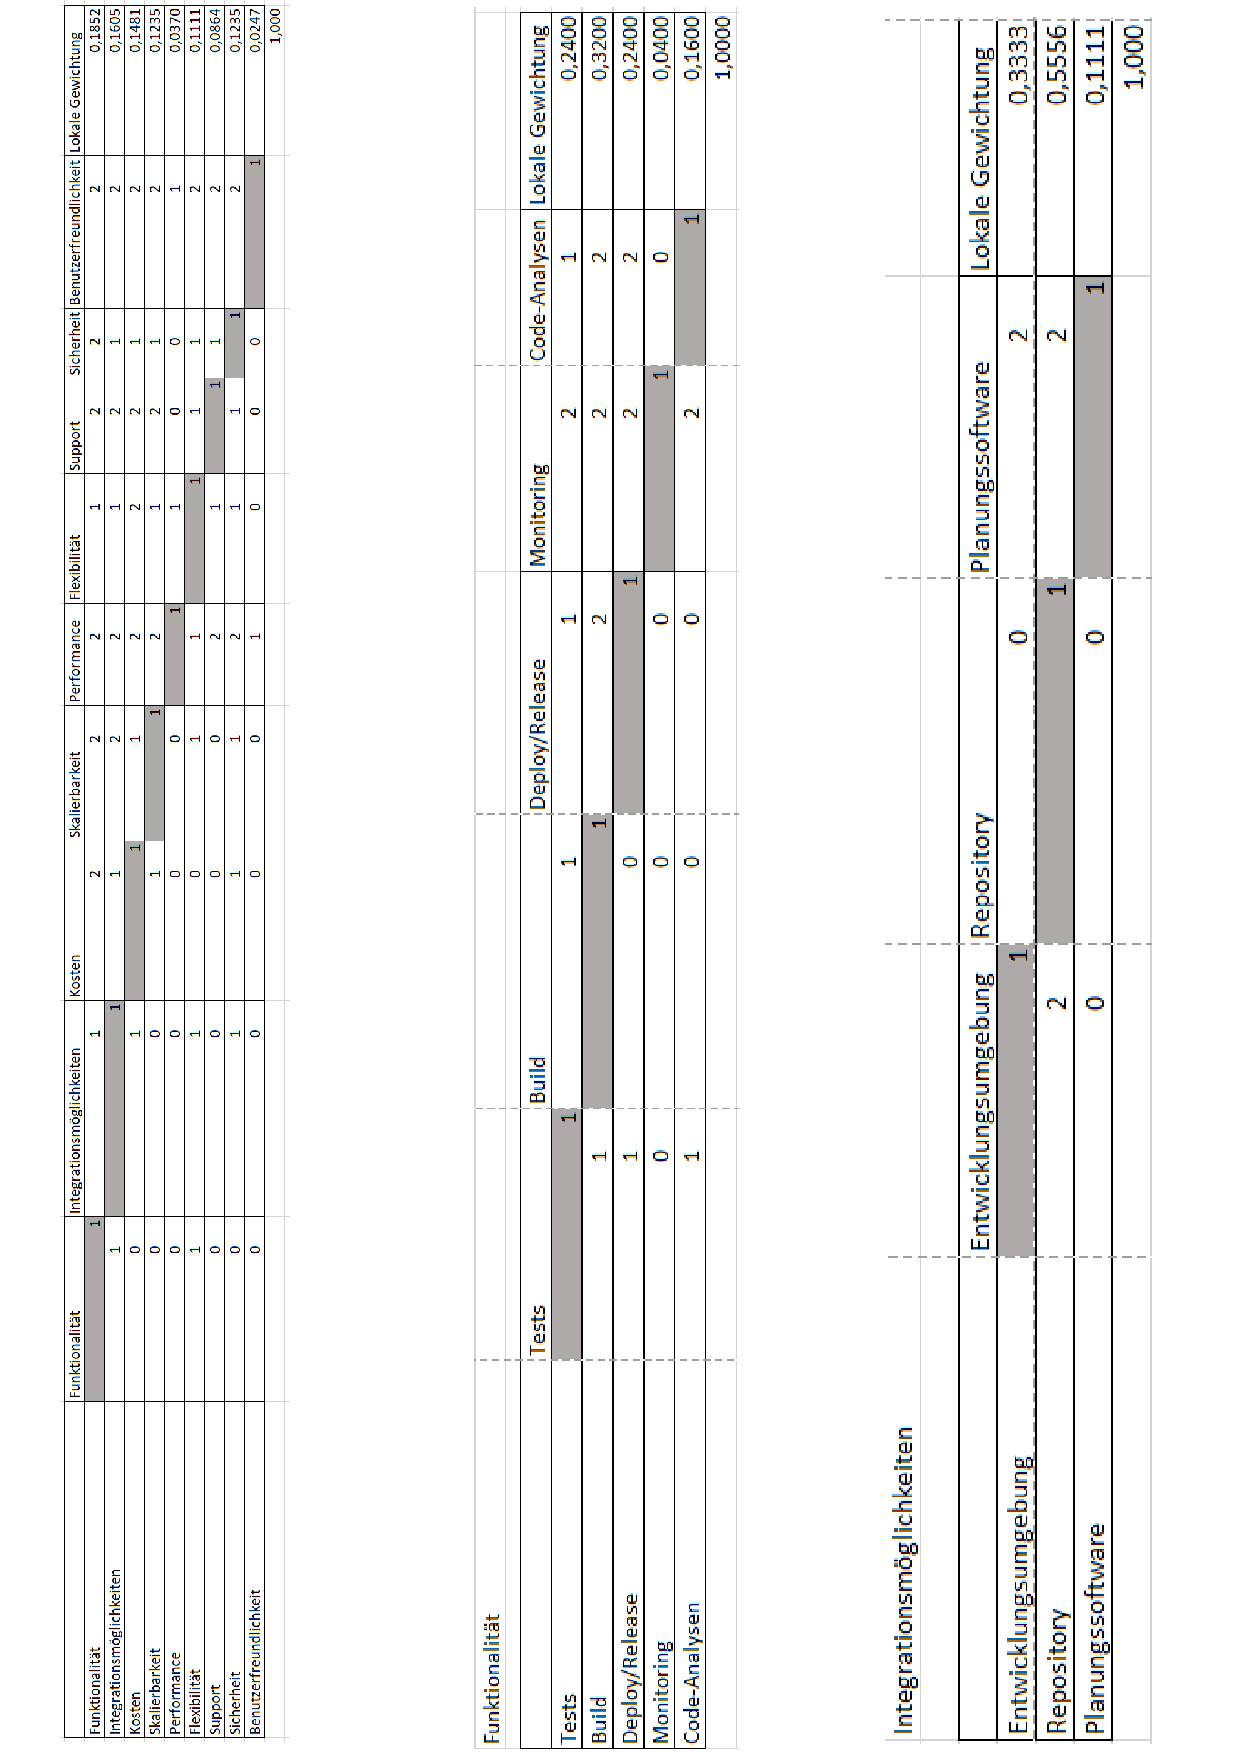
\includegraphics{Soelker_1}}
            \label{fig:CEA}
        \end{figure}	
    \end{center}
    \begin{center}
        \begin{figure}[H]
            \centering
            \scalebox{0.7}{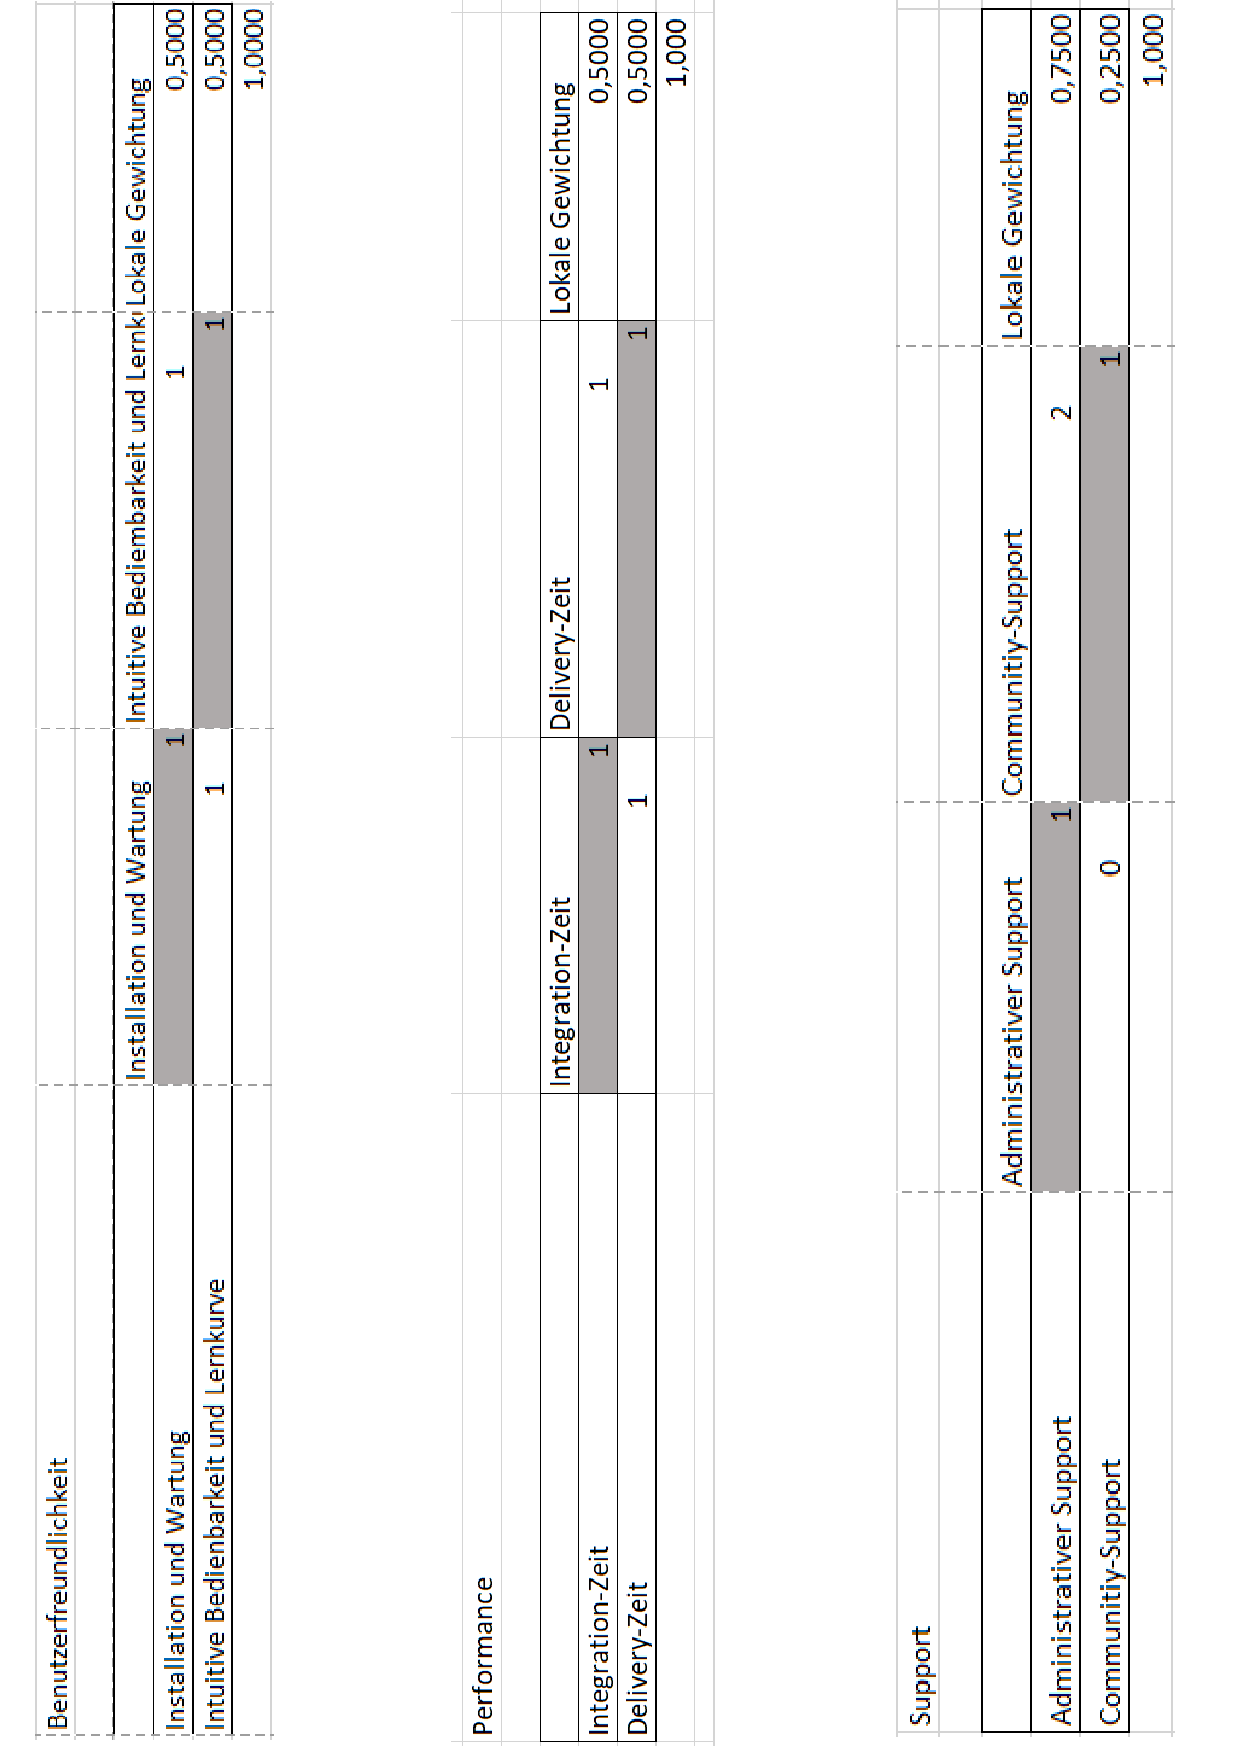
\includegraphics{Soelker_2}}
            \label{fig:CEA}
        \end{figure}	
    \end{center}

    \begin{center}
        \begin{figure}[H]
            \centering
            \scalebox{0.7}{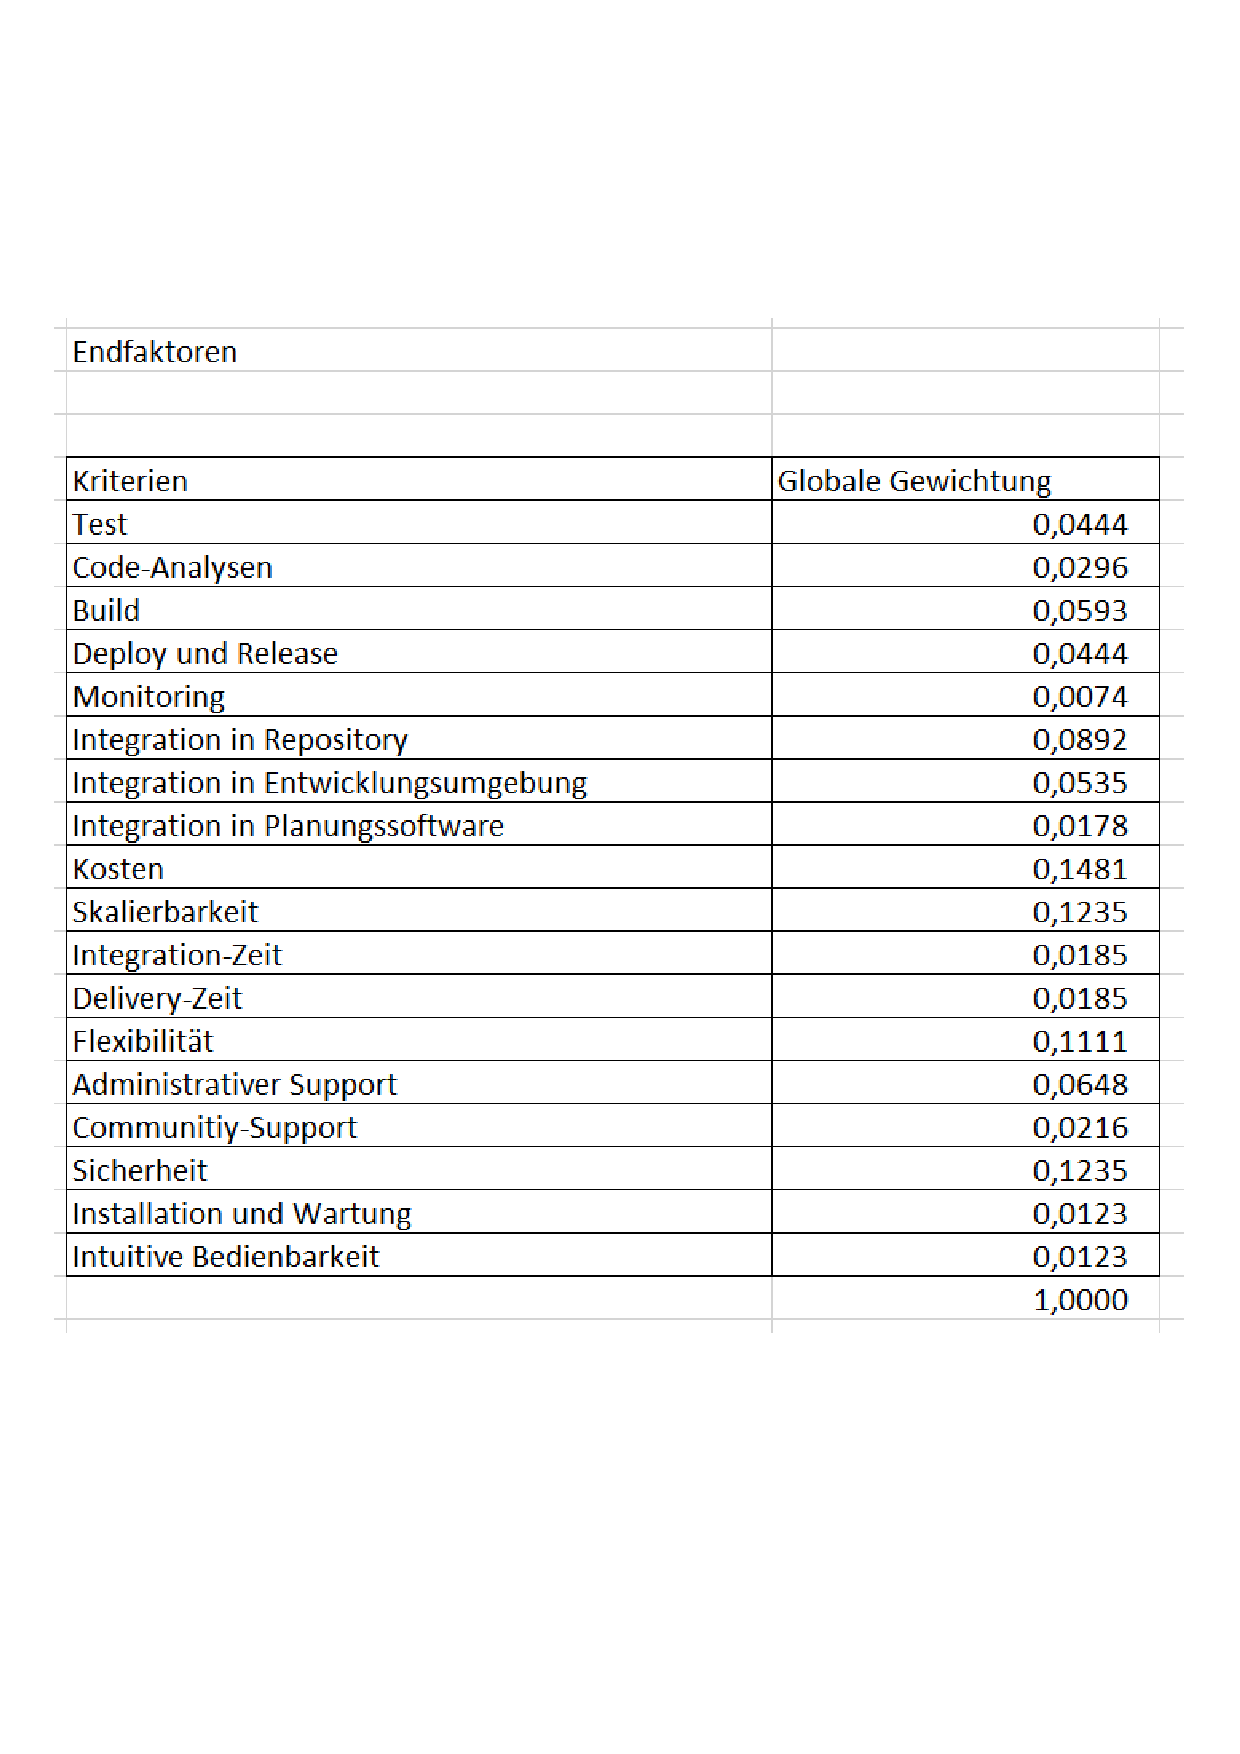
\includegraphics{Soelker_3}}
            \label{fig:CEA}
        \end{figure}	
    \end{center}
    \newpage
    \resetlinenumber
    \begin{linenumbers}
        \textbf{Interviewer:} Für dich besonders wichtig ist die Funktionalität. Kannst du das begründen?\\
        \textbf{Experte:} Wenn ich eine Pipeline einbaue, dann ist für mich besonders wichtig, dass die Pipeline bestimmte Funktionalitäten, wie z.B. Tests abdecken. Weniger gewichtig ist da z.B. die Benutzerfreundlichkeit. Ich bin der Meinung, dass ich eine Pipeline einmal einrichte. Da spielt es dann auch weniger die Rolle wie viel Aufwand das beim initialen Einrichten war.\\
            \textbf{Interviewer:} Von den Subkriterien der Funktionalität war für dich Build Funktionalität besonders wichtig. Kannst du das begründen?\\
            \textbf{Experte:} Bei Cloud-Native-Projekten werden i.d.R. verschiedene Sprachen und verschiedene Frameworks verwendet. Die Pipeline sollte da einfach alle Build-Packages unterstützen. So muss ich dann nicht hergehen und manuell irgendwelche Deployments ausführen. Tests waren für mich auch sehr wichtig. Es ist wichtig, dass ich die Tests mache, bevor es zu Merges kommt. Natürlich kann ich auch Tests abseits von einer CI/CD-Pipeline ausführen. Bei einem größeren Team von Entwickler ist das jedoch kaum noch kontrollierbar.\\
            \textbf{Interviewer:} Kommen wir zu den Integrationsmöglichkeiten. Deiner Meinung nach ist die Integration eines Repositorys sehr wichtig. Woran liegt das?\\
            \textbf{Experte:} Oft ist es so, dass sich der Kunde auf eine oder zwei CI/CD und ein oder zwei Repositorys einschießt. Gerade, wenn da die Abhängigkeit mit dem Repository besteht sollte das natürlich in die CI/CD-Pipeline integrierbar sein.\\
            \textbf{Interviewer:} Kannst du begründen, warum für dich die Integration- und Delivery-Zeit gleich wichtig ist.\\
            \textbf{Experte:} Aus meiner Sicht gibt es da kein wichtigeres Kriterium, da sowohl CI als auch CD im Hintergrund läuft. Somit ist es für mich jetzt nicht so wichtig, falls eine der beiden Pipelines länger durchläuft.\\
            \textbf{Interviewer:} Warum ist für dich der administrative Support wichtiger als der Community-Support?\\
            \textbf{Experte:} Für mich ist es eben sehr wichtig, dass es eine gute Dokumentation gibt. So kann ich z.B. bevor ich eine Pipeline installiere schon abschätzen, wie gut bestimmte Aspekte funktioniere und bin da nicht davon abhängig, dass ich durch Community-Foren irgendwelche Workarounds bekomme. Außerdem ist es mir natürlich auch sher wichtig, dass die Lösung immer auf dem neusten Stand der Technik ist.\\
            \textbf{Interviewer:} Sowohl Sicheheitsarchitektur als auch Authentifizierung- und Autorisierungskonzepte sind dir gleich wichtig. Kannst du das begründen?\\
            \textbf{Experte:} Also es gehört natürlich einfach zur Developer-Experience dazu, wenn man bestimmte Authentifizierung- und Autorisierungskonzepte hat. Dann ist es natürlich aber auch schon wichtig, dass die Pipeline an sich sicher ist. Gerade die Pipeline bietet natürlich eine sehr gute Möglichkeit feindliche Programme in eine Produktionsumgebung einzuführen.\\
    \end{linenumbers}
    

    
    \newpage
    \subsection{Expertengewichtung 2}
            \begin{tabular}{ l l }
        Interviewpartner: & Full-Stack-Entwickler SAP DTS Integration (Experte 6)\\
        Datum: & 21.03.2023\\
        Interview-Medium: & Microsoft-Teams\\
\end{tabular}
\begin{center}
    \begin{figure}[H]
        \centering
        \scalebox{0.6}{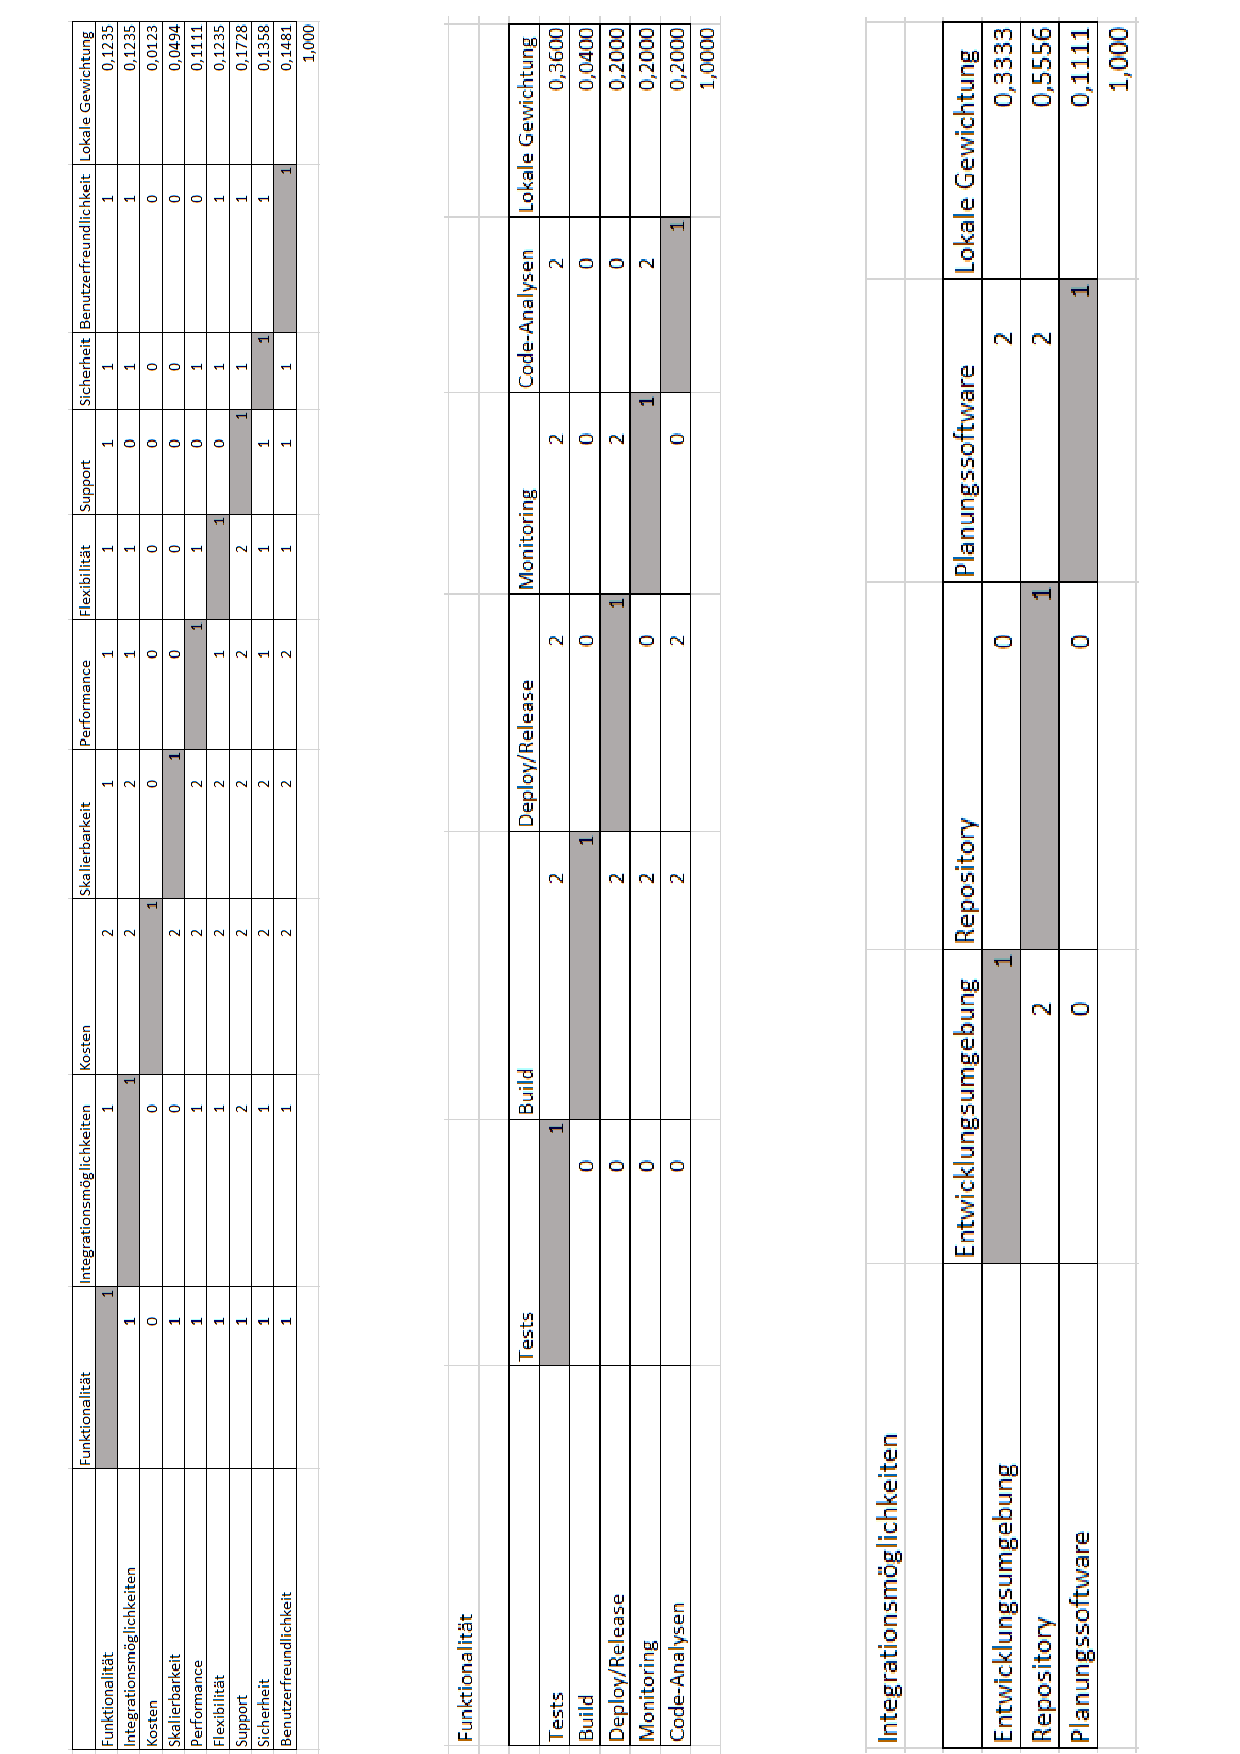
\includegraphics{Trump_1}}
        \label{fig:CEA}
    \end{figure}	
\end{center}
\begin{center}
    \begin{figure}[H]
        \centering
        \scalebox{0.7}{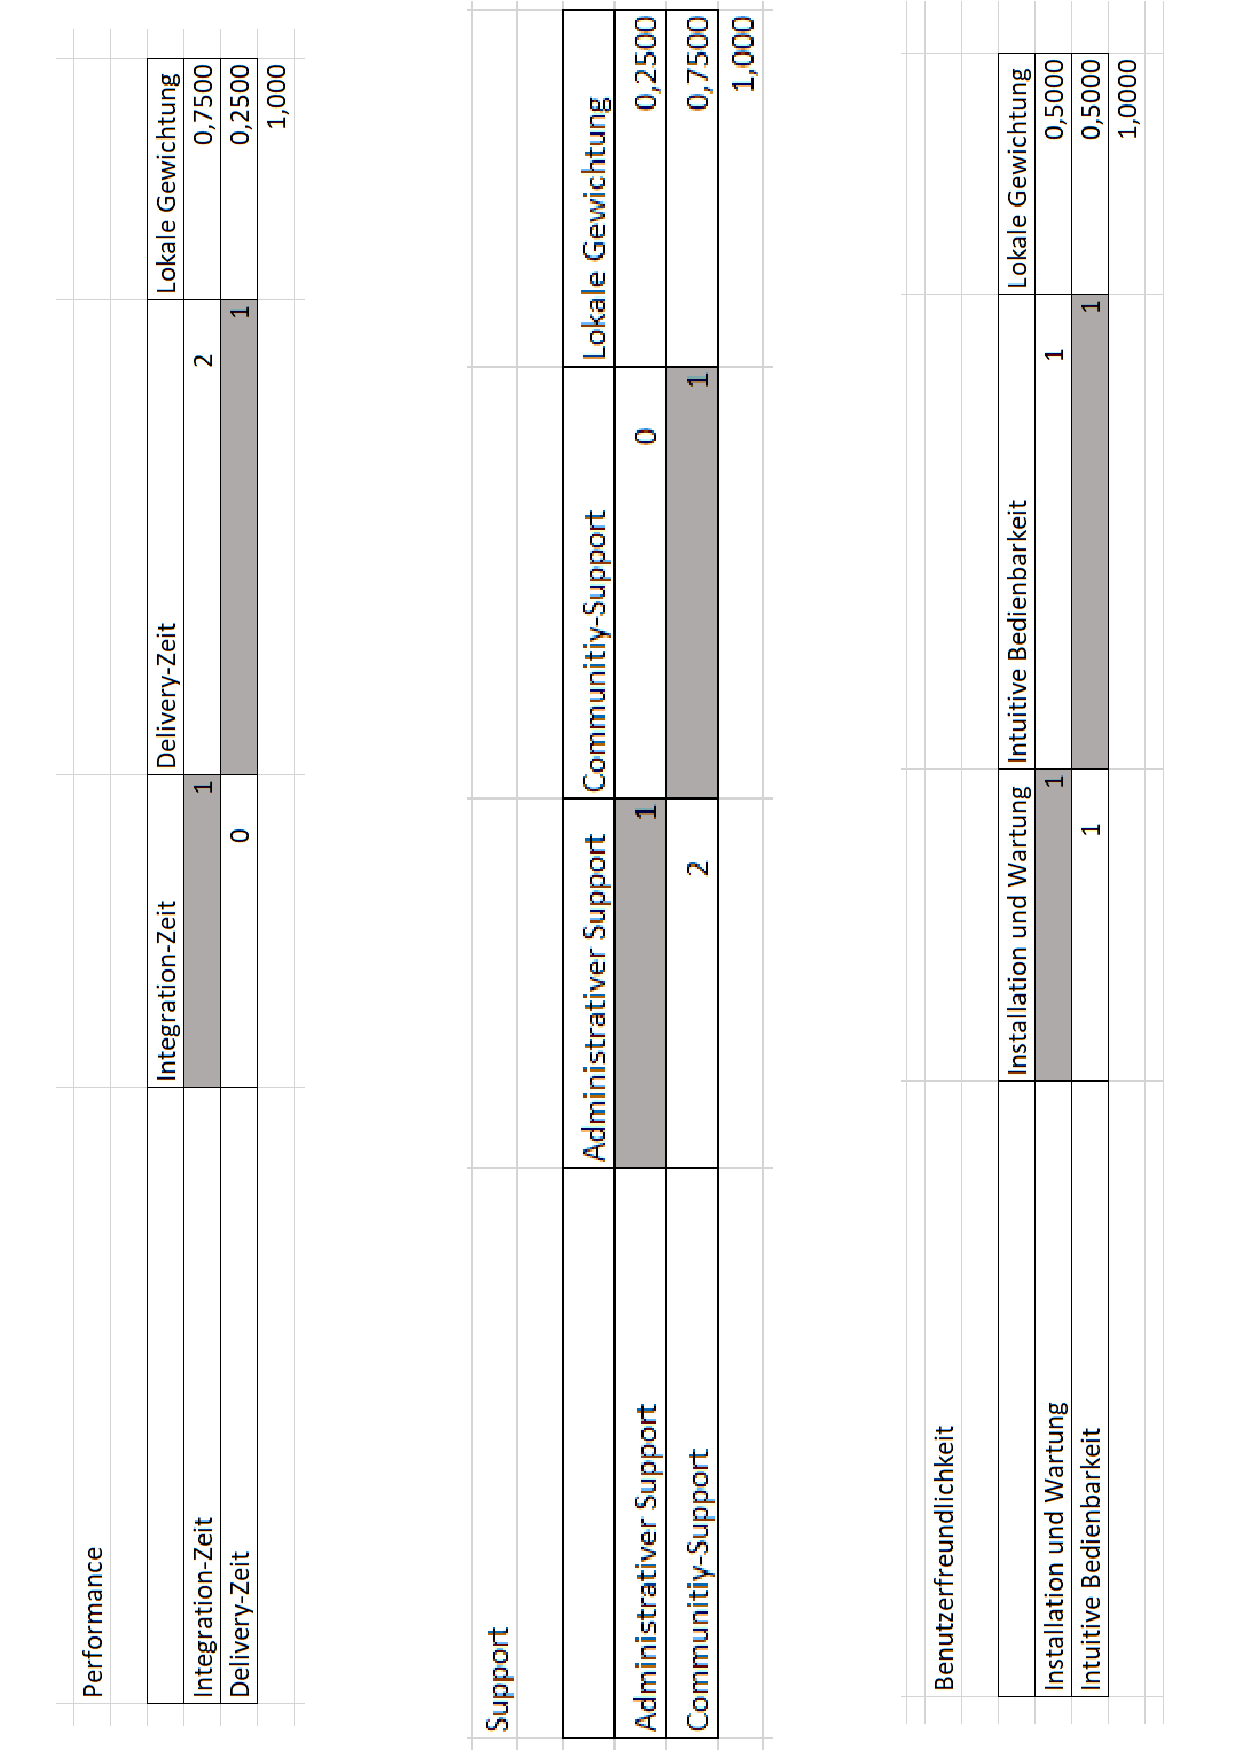
\includegraphics{Trump_2}}
        \label{fig:CEA}
    \end{figure}	
\end{center}

\begin{center}
    \begin{figure}[H]
        \centering
        \scalebox{0.7}{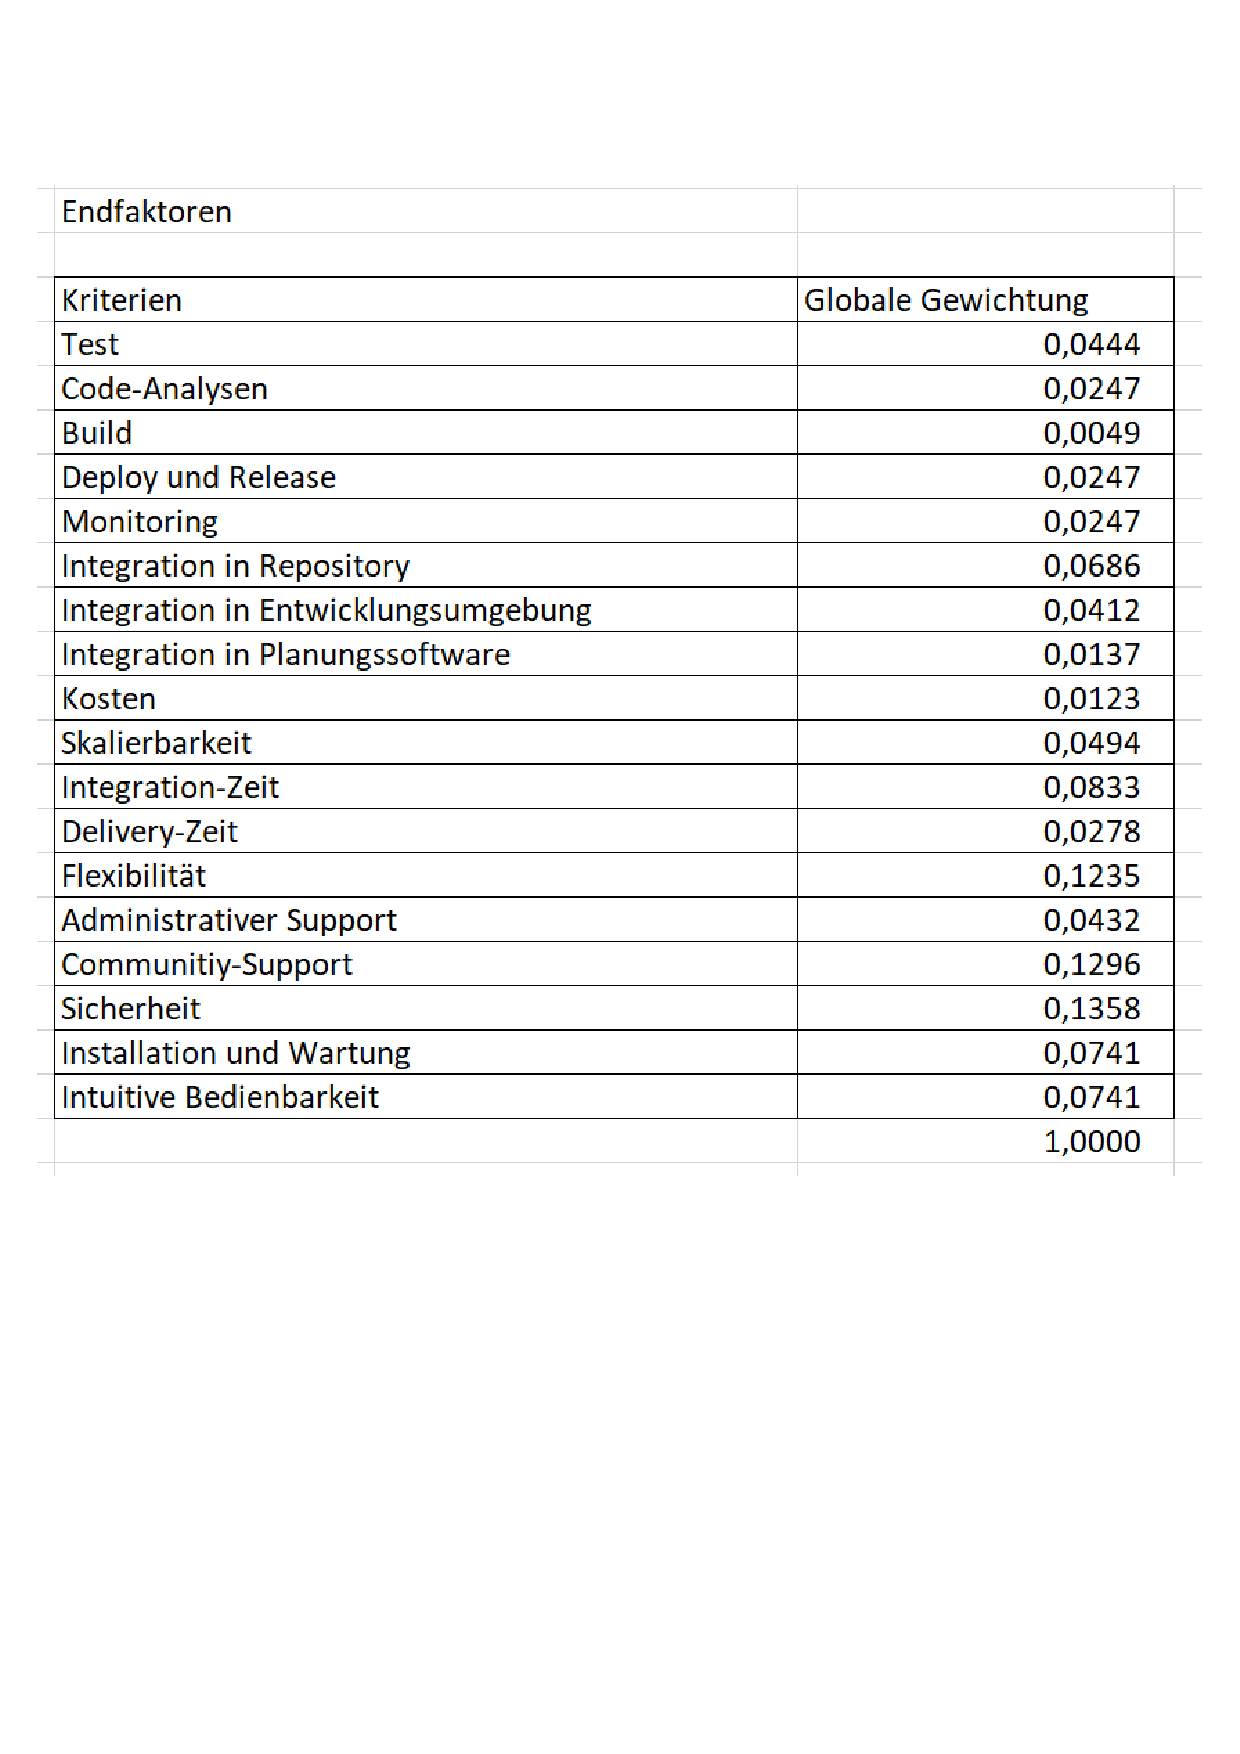
\includegraphics{Trump_3}}
        \label{fig:CEA}
    \end{figure}	
\end{center}
\newpage

\resetlinenumber
\begin{linenumbers}
    \textbf{Interviewer}: In Tabelle 1 ist für dich besonders wichtig der Support und weniger wichtig sind für dich die Kosten. Warum?\\
    \textbf{Experte}: Ich als Entwickler habe die Erfahrung, dass Tool noch so toll sein kann. Wenn keine gute Dokumentation vorhanden ist, dann hilft mir das als Entwickler nicht viel. Die Kosten sind mir aus Entwicklersicht egal. Da sind mir erstmal die anderen Kriterien wichtiger\\
    \textbf{Interviewer}: In Tabelle 2 waren dir die Tests besonders wichtig. Kannst du das begründen.\\
    \textbf{Experte:} Es spart mir sehr viel Zeit, wenn Tests automatisiert werden. Für mich gehört das automatisierte Ausführen von Tests auch zu den Hauptzwecken einer CI/CD-Pipeline. So kann ich frühzeitig erkennen, wenn eine Änderung etwas kaputt macht.\\
    \textbf{Interviewer:} Kommen wir zu den Integrationsmöglichkeiten. Warum ist dir die Integration in Repositorys besonders wichtig?\\
    \textbf{Experte:} Ich sehe, dass als eine sehr grundlegende Funktion. Wenn meine CI/CD-Pipeline nicht mit dem Repository integrierbar ist, dann wird das gesamte Konzept einer Pipeline hinfällig. Die Planungssoftware war mir hingegen kaum wichtig, da ich als Entwickler mit so etwas kaum arbeite.\\
    \textbf{Interviewer:} Kannst du deine Entscheidungen zur Performance begründen?\\
    \textbf{Experte:} Für mich ist die Integration-Zeit deutlich wichtiger, einfach um da eine höhere Developer-Experience zu bekommen. Wenn ich ein Pull-Request aufmache, dann möchte ich auch schnell Feedback bekommen, ob alles passt oder eben nicht.\\
    \textbf{Interviewer:} Kannst du deine Entscheidungen zum Support begründen?\\
    \textbf{Experte:} Ich finde den Community-Support am wichtigsten. Dabei bekommt man den leichtesten Zugriff als Entwickler auf neues Wissen. Weniger geeignet fände ich, wenn ich jedes Mal mit jemanden telefonieren müsste oder immer ein neues Ticket aufmachen müsste. Weiterhin ist es sehr gut, wenn von einer Community Plug-ins bereitgestellt werden. Damit kann ich den Funktionsumfang erweitern. Jedoch besteht hier immer die Gefahr, dass Plug-ins Sicherheitslücken besitzen oder irgendwann nicht mehr richtig gewartet werden können.\\
    \textbf{Interviewer:} Wie sieht es mit dem Punkt der Sicherheit aus?\\
    \textbf{Experte:} Ich finde das Authentifizierungs- und Autorisierungs-Konzept am wichtigsten, da dies auch mit der Developer-Experience zusammenhängt. Damit komme ich eben in meinem Entwickleralltag am meisten in Berührung. Wenn die Plattform bspw. SSO enabled ist, dann ist das für mich als Programmierer sehr gemütlich.\\ 
    \textbf{Interviewer:} Kannst du deine Entscheidung zur Benutzerfreundlichkeit begründen?\\
    \textbf{Experte:} Sowohl mit Wartung bzw. Installation und mit der gewöhnlichen Bedienbarkeit kommt man gelegentlich in Berührung. Das sollte deshalb beides einigermaßen gut funktionieren.\\
\end{linenumbers}

\newpage
\subsection{Expertengewichtung 3}
        \begin{tabular}{ l l }
    Interviewpartner: & Test Developer SAP Hyperspace Adoption \& Onboarding (Experte 4)\\
    Datum: & 22.03.2023\\
    Interview-Medium: & Microsoft-Teams\\
\end{tabular}
\begin{center}
\begin{figure}[H]
    \centering
    \scalebox{0.6}{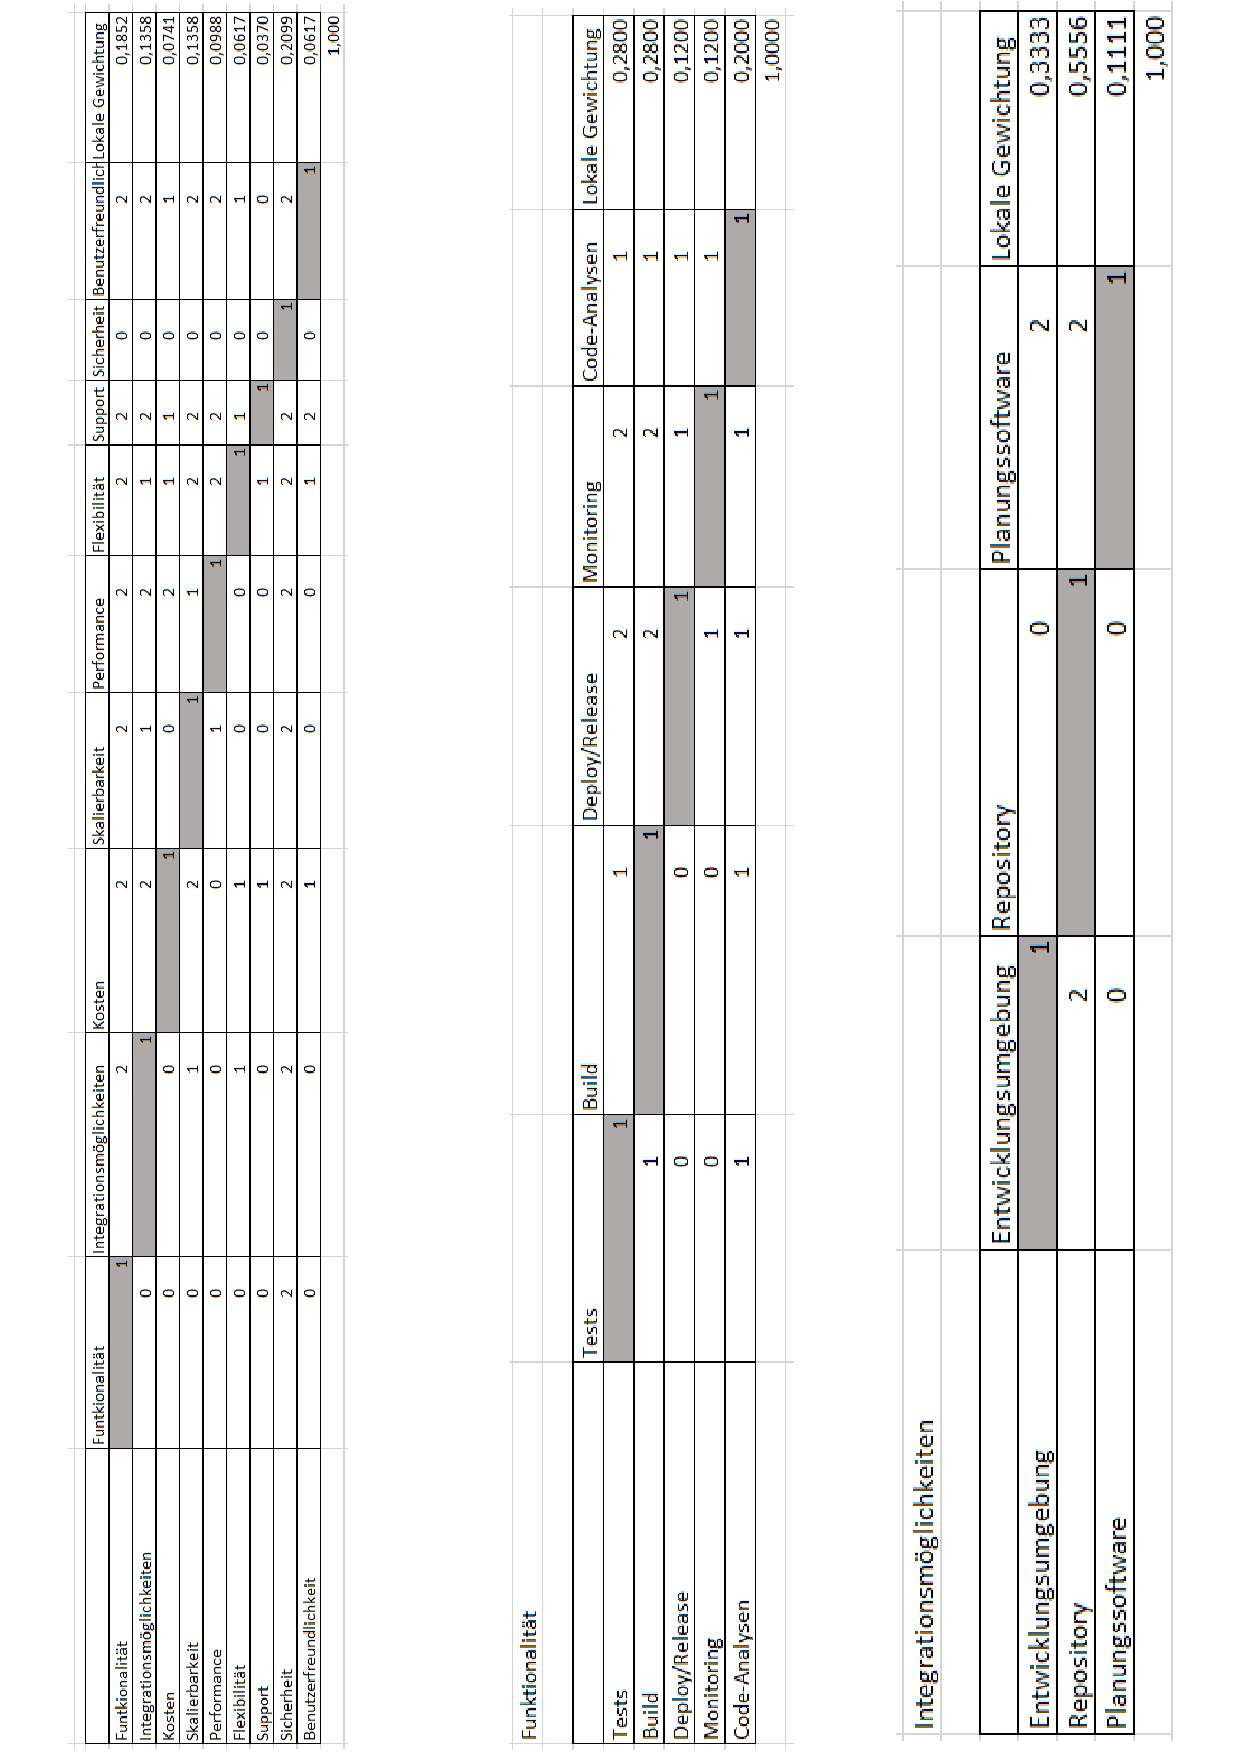
\includegraphics{Bischoff_1}}
    \label{fig:CEA}
\end{figure}	
\end{center}
\begin{center}
\begin{figure}[H]
    \centering
    \scalebox{0.7}{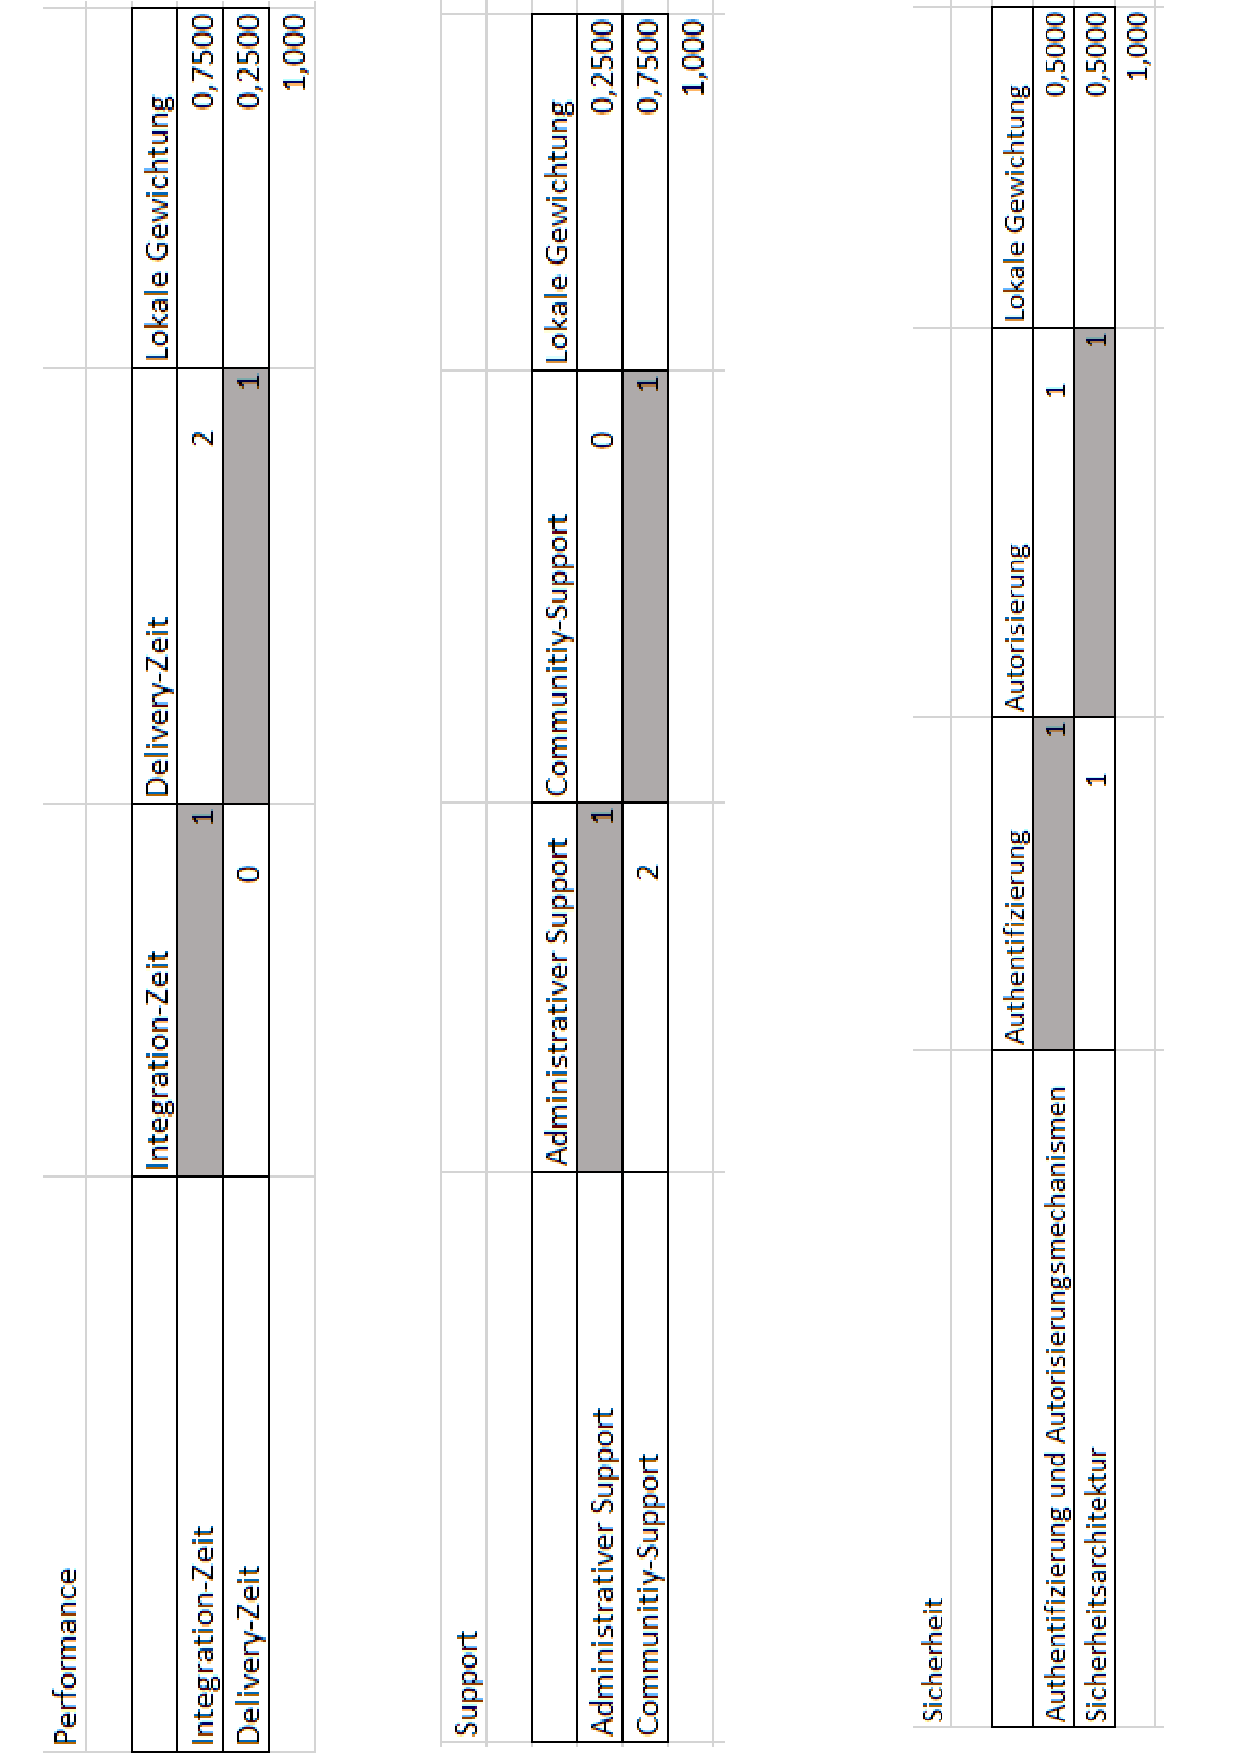
\includegraphics{Bischoff_2}}
    \label{fig:CEA}
\end{figure}	
\end{center}

\begin{center}
\begin{figure}[H]
    \centering
    \scalebox{0.7}{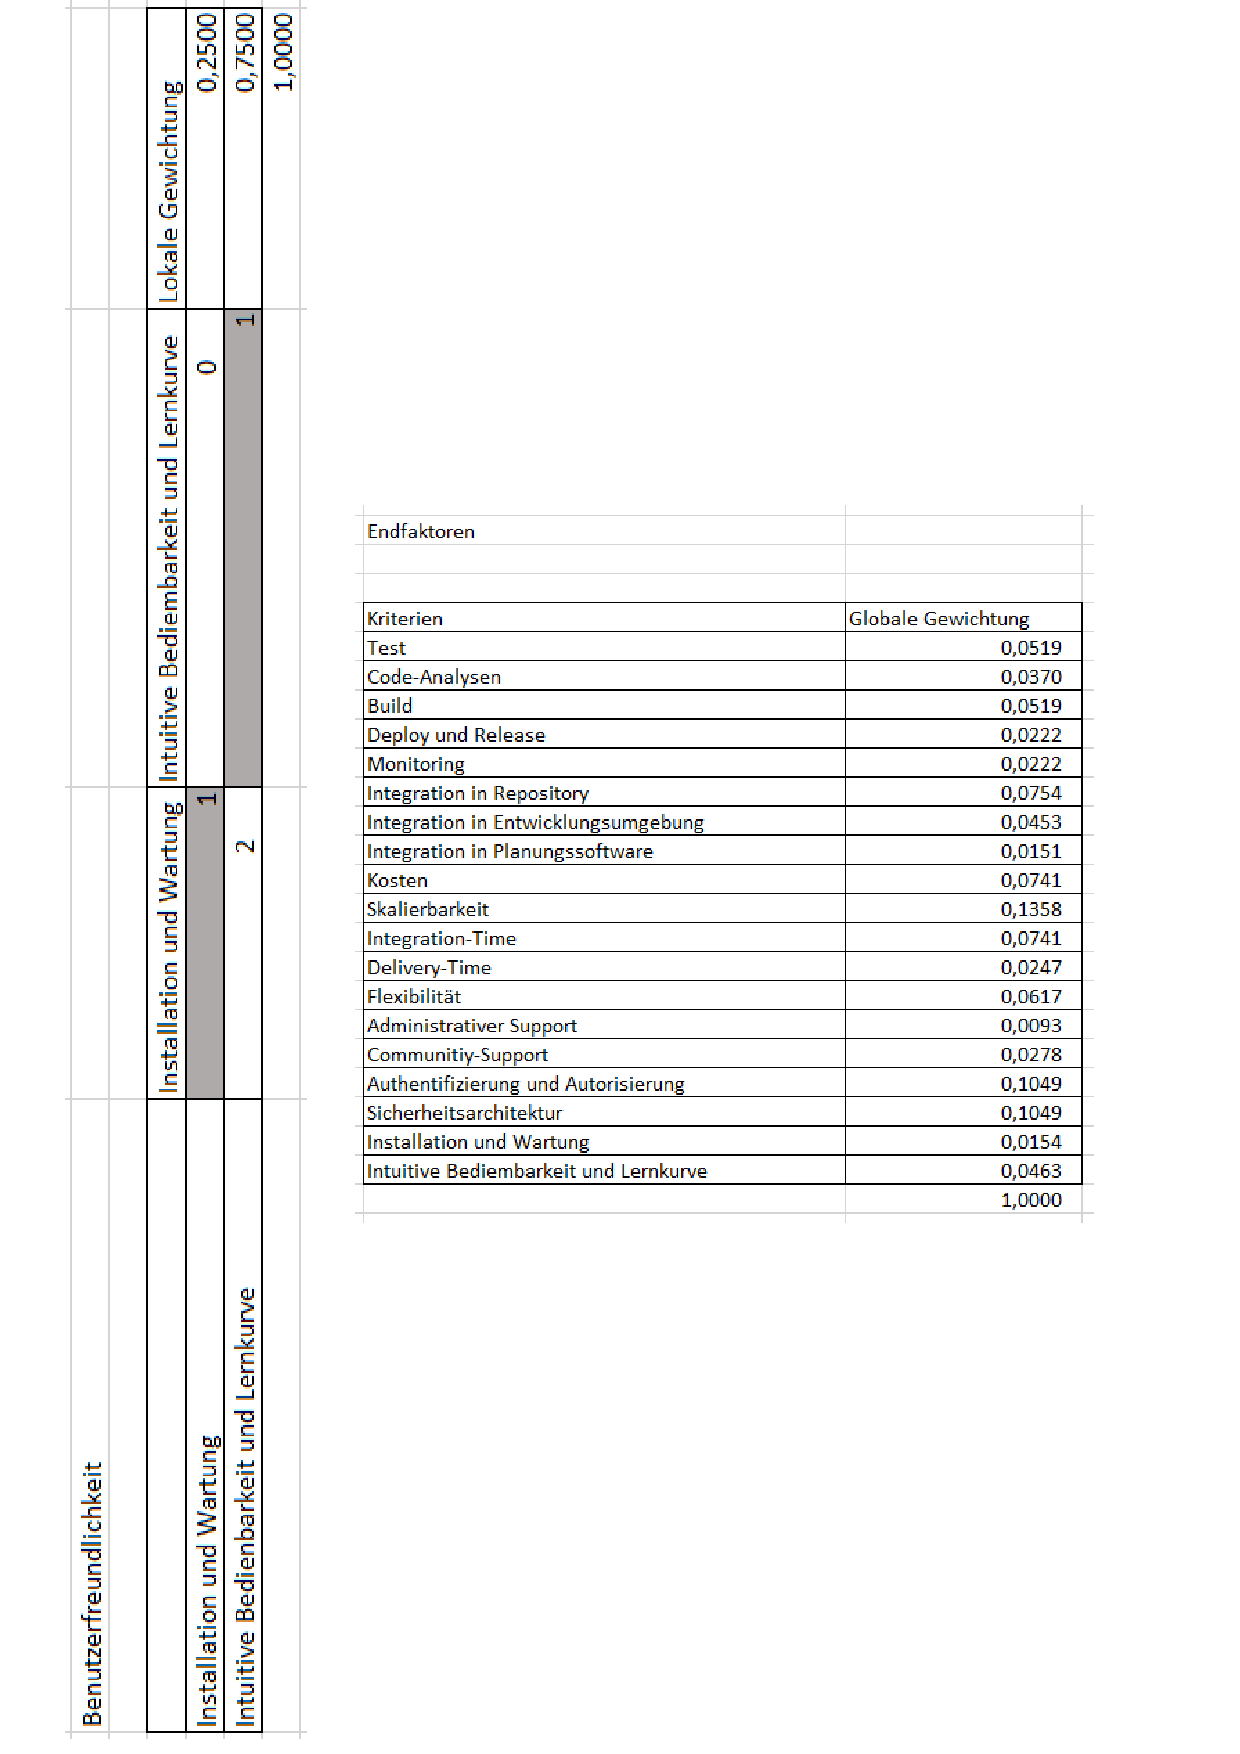
\includegraphics{Bischoff_3}}
    \label{fig:CEA}
\end{figure}	
\end{center}
\newpage
\resetlinenumber
\begin{linenumbers}
    \textbf{Interviewer:} Besonders wichtig ist für dich die Sicherheit. Kannst du das begründen?\\
    \textbf{Experte:} Sicherheitslücken in unseren Systemen würden einen sehr großen Imageschaden verursachen. Deswegen ist das für mich das absolute Top-Thema. Gerade wenn wir neue Software bereitstellen, darf es nicht passieren, dass eventuell feindliche Programme eingeschleust werden. Nicht so wichtig ist für mich der Support, da dieser ganz schnell zum Bottleneck werden kann. Wichtiger ist da für mich z.B. die Benutzerfreundlichkeit. Man sollte die Nutzer gar nicht erst in die Situation kommen lassen, dass diese Support benötigen.\\
    \textbf{Interviewer:} Warum ist für dich der administrative Support wichtiger als der Community-Support?\\
    \textbf{Experte:} Es ist viel wichtiger, dass man eine Community besitzt, welche Fragen beantworten kann. Dies ist eigentlich die einzige Möglichkeit sowas skalierbar zu machen. Man wird niemals ein Support-Team besitzen, was groß genug ist alle Fragen zu beantworten. Man könnte den administrativen Support also nicht gut skalieren.\\
    \textbf{Interviewer:} Im Kriterium der Funktionalität ist für dich besonders wichtig die Test- und Build-Funktionalität. Warum?\\
    \textbf{Experte:} Test ist natürlich mein Hintergrund, da ich von dieser Seite her komme. Es ist für mich einfach wichtig, dass ich etwas ausliefere, was auch validiert ist. 
    \textbf{Interviewer:} Warum ist für dich die Integration-Zeit wichtiger als die Delivery-Zeit?\\
    \textbf{Experte:} Es kann eben aus Entwicklersicht nicht sein, dass ich eine Änderung im Code mache und dann erst einmal eine halbe Stunde warten muss, bis ich Feedback bekomme. Da geht die Motivation im Team verloren. Und es stapeln sich einfach die Änderungen, bevor ich die Änderungen dann tatsächlich ausliefere.\\
    \textbf{Interviewer:} Für sind sowohl Authentifizierung bzw. Autorisierung und die Sicherheitsarchitektur gleich wichtig. Kannst du das begründen?\\
    \textbf{Experte:} Authentifizierung ist natürlich wichtig, damit nicht jemand unberechtigtes ein Deployment durchführen kann, welcher das eigentlich gar nicht sollte.\\
    \textbf{Interviewer:} Für dich war die Installation und Wartung weniger wichtig als die intuitive Bedienbarkeit?\\
    \textbf{Experte:} Installation und Wartung betrifft mich einmal beim Setup, während die intuitive Bedienbarkeit kontinuierlich wichtig ist.\\
\end{linenumbers}

